\documentclass[11pt,a4paper]{article}
\usepackage{isabelle,isabellesym, amsmath}
\usepackage{times}
\usepackage{graphicx}
\usepackage{natbib}
\bibliographystyle{abbrvnat}
\setcitestyle{authoryear,open={(},close={)}}

\normalfont
\setlength\parindent{24pt}
\newcommand{\isactrlemph}[1]{\emph{#1}}
\usepackage{setspace}
\doublespacing

% further packages required for unusual symbols (see also
% isabellesym.sty), use only when needed

\usepackage{amssymb}
  %for \<leadsto>, \<box>, \<diamond>, \<sqsupset>, \<mho>, \<Join>,
  %\<lhd>, \<lesssim>, \<greatersim>, \<lessapprox>, \<greaterapprox>,
  %\<triangleq>, \<yen>, \<lozenge>

%\usepackage{eurosym}
  %for \<euro>

%\usepackage[only,bigsqcap]{stmaryrd}
  %for \<Sqinter>

%\usepackage{eufrak}
  %for \<AA> ... \<ZZ>, \<aa> ... \<zz> (also included in amssymb)

%\usepackage{textcomp}
  %for \<onequarter>, \<onehalf>, \<threequarters>, \<degree>, \<cent>,
  %\<currency>

% this should be the last package used
\usepackage{pdfsetup}

% urls in roman style, theory text in math-similar italics
\urlstyle{rm}
\isabellestyle{it}

% for uniform font size
%\renewcommand{\isastyle}{\isastyleminor}


\begin{document}

\title{Philosophical Writing}
\author{Lavanya Singh}
\maketitle
\tableofcontents


\newpage

% sane default for proof documents
\parindent 0pt\parskip 0.5ex

% generated text of all theories
%
\begin{isabellebody}%
\setisabellecontext{threeflags}%
%
\isadelimtheory
%
\endisadelimtheory
%
\isatagtheory
%
\endisatagtheory
{\isafoldtheory}%
%
\isadelimtheory
%
\endisadelimtheory
%
\isadelimdocument
%
\endisadelimdocument
%
\isatagdocument
%
\isamarkupsection{Choice to Formalize the FUL%
}
\isamarkuptrue%
%
\endisatagdocument
{\isafolddocument}%
%
\isadelimdocument
%
\endisadelimdocument
%
\begin{isamarkuptext}%
In \emph{Groundwork of the Metaphysics of Morals}, Kant presents three formulations, or versions, 
of what he calls the ``supreme law of morality." I will focus on the first of these three formulations, 
and below I explain the formulations and defend my choice.

Kant argues that if  morality 
exists, it must take the form of a categorical imperative or a law that holds unconditionally. Categorical
imperatives are contrasted with hypothetical imperatives, which take the form of conditionals as in, 
``If I want to get good grades, I must study hard." Hypothetical imperatives only have force so long
as the antecedent holds, but the categorical imperative is unconditionally binding \cite[28]{groundwork}. In the first 
half of \emph{Groundwork}, Kant examines what the categorical imperative, if such a thing exists and has force,
must be. He concludes that there are three ``formulations" of the categorical imperative, or three ways 
of articulating the supreme law of morality. 

The first formulation of the categorical imperative is the
formula of universal law (FUL), which reads, ``act only according to that maxim through which you can 
at the same time will that it become a universal law." \cite[34]{groundwork} This formulation
generates the universalizability test, which ``tests" the moral value of a maxim by 
imagining a world in which it becomes a universal law and attempting to will the maxim in that world. The 
second formulation of the categorical imperative is the formula of humanity (FUH): ``So act that you use humanity, 
in your own person, as well as in the person of any other, always at the same time as an end, never merely 
as a means." \cite[41]{groundwork}. This formulation is often understood as requiring us to 
acknowledge and respect the dignity of every other person. The third formulation of the categorical 
imperative is the formula of autonomy (FOA), which Korsgaard summarizes in her introduction to the Groundwork 
as, ``we should so act that we may think of ourselves as legislating universal laws through our 
maxims" \cite[28]{korsgaardintro}. While closely related to the FUL, the FOA presents morality as the activity of 
perfectly rational agents in an ideal ``kingdom of ends," guided by what Kant calls the ``laws of freedom."

I choose to focus on formalizations of Kant's first formulation of the categorical imperative,
the formula of universal law (FUL), because it is the most formal and thus the easiest to formalize and implement. 
Onora O'Neill explains that the formalism of the FUL allows 
for greater precision in philosophical arguments analyzing its implications and power \cite[33]{actingonprinciple}. This precision 
is particularly useful in a computational context because any formalism necessarily makes its content 
precise. The FUL's existing precision reduces ambiguity, allowing me to remain faithful to Kant's writing and 
philosophical interpretations of it. Precision reduces the need to make choices to resolve debates 
and ambiguities. Some of these choices may be well-studied and grounded in literature, 
but some may be unique to formalizing the FUL and thus understudied. Minimizing these choices minimizes 
arbitrariness in my formalization and puts it on solid philosophical footing. Given that this thesis is a proof-of-concept, 
the formalism of the FUL is attractive because it reduces both the computational and philosophical complexity of my work. 

While some criticize the FUL for its formalism and percieved ``sterility" \cite[33]{actingonprinciple}, 
Kantian constructivists embrace it \cite[173]{ebelsduggan}. My project is not committed to Kantian constructivism. 
I believe that computational ethics is likely a valuable tool for any ethicist, and I make the case 
for Kantian ethics specifically. Nonetheless, Kantian constructivists may find the focus on 
the FUL particularly appealing. 

Though Kantians study all formulations of the categorical imperative, Kant argues in Groundwork 
that the three formulations of the categorical imperative are equivalent \cite{groundwork}. While this 
argument is disputed \cite{sepkant}, for those who believe it, the
stakes for my choice of the FUL are greatly reduced. If all formulations are equivalent, then a formalization of the FUL
lends the exact same power as a formalization of the second or third formulation of the categorical 
imperative. In fact, future work could formalize the other formulas and try to prove that they 
are identical. Kant believes that his argument for the equality of the formulas is analytical, and
if he is correct, it should be possible to recreate the argument in logic.%
\end{isamarkuptext}\isamarkuptrue%
%
\isadelimdocument
%
\endisadelimdocument
%
\isatagdocument
%
\isamarkupsection{Definition of a Maxim%
}
\isamarkuptrue%
%
\endisatagdocument
{\isafolddocument}%
%
\isadelimdocument
%
\endisadelimdocument
%
\begin{isamarkuptext}%
The central unit of evaluation for the universalizability test is a ``maxim," which Kant defines 
in a footnote in \emph{Groundworkd} as ``the subjective principle of willing," or the principle that 
the agent acts on \cite[16]{groundwork}. Modern Kantians differ in their interpretations of this definition. The naive view 
is that a maxim is an act, but Korsgaard adopts the more sophisticated view that a maxim is composed
of an act and the agent's purpose for acting \cite{actingforareason}. She also compares a maxim 
to Aristotle's logos, which includes these components and information about the circumstances and methods 
of the act. O'Neill concludes that Kant's examples imply that a maxim must also include circumstances \cite{actingonprinciple}, and 
Kitcher \cite{whatisamaxim} uses textual evidence from the Groundwork to argue for the inclusion of a maxim's purpose 
or motivation. In order to formalize the notion of a maxim, I must adopt a specific definition and 
defend my choice.

I define a maxim as a circumstance, act, goal tuple (C, A, G), read 
as ``In circumstances C, act A for goal G." Isabelle's strict typing rules mean that the choice of the 
type of each member of this tuple is significant. A circumstance is represented as a set of worlds 
$t$ where that circumstance holds. A goal is also a term because it can be true or false at a world if it 
is realized or not. An act is an open sentence because an act itself is not the kind of thing that can 
be true or false (as in, an act is not truth-apt), but the combination of a subject performing an act 
can be true or false at a world depending on whether or not the act is indeed performed by that subject. 
For example, ``running" is not truth-apt, but ``Sara runs" is truth-apt.

My definition of a maxim is inspired by O'Neill's work on maxims. I will defend my representation
below and consider an additional component that Kitcher argues for.%
\end{isamarkuptext}\isamarkuptrue%
%
\isadelimdocument
%
\endisadelimdocument
%
\isatagdocument
%
\isamarkupsubsection{O'Niell's Original Schematic and The Role of Practical Judgement%
}
\isamarkuptrue%
%
\endisatagdocument
{\isafolddocument}%
%
\isadelimdocument
%
\endisadelimdocument
%
\begin{isamarkuptext}%
O'Neill \cite[37]{actingonprinciple} presents what Kitcher \cite{whatisamaxim}  calls the widely accepted 
view that a maxim is a circumstance, act, goal tuple. A maxim 
is an action-guiding rule and thus naturally includes an act and the circumstances under which 
it should be performed, which are often referred to as ``morally relevant circumstances." 

She also includes a purpose, end, or goal in the maxim because Kant includes this in many of his 
example maxims and because Kant argues that human activity, because it is guided by a rational will, 
is inherently purposive \cite[4:428]{groundwork}. A rational will does not act randomly (else it would not be rational), 
but instead in the pursuit of ends which it deems valuable. This inclusion is also essential for the version of the universalizability test 
that I will implement, explained in Section ??.

O'Neill's inclusion of circumstances is potentially controversial because it leaves open the question of what qualifies as a 
relevant circumstance for a particular maxim. This is gives rise to ``the tailoring objection" \cite[217]{whatisamaxim} \footnote{Kitcher
cites \cite{kantsethicalthought}  as offering an example of a false positive due to this objection.}, 
under which maxims are arbitrarily specified to pass the FUL. For example, the maxim ``When my name is Lavanya Singh,
I will lie to get some easy money," is universalizable, but is clearly a false positive. One solution to 
this problem is to argue that the circumstance ``When my name is Lavanya Singh" is not morally relevant 
to the act and goal. This solution requires some discussion of what qualifies as a relevant circumstance.

O'Neill seems to acknowledge the difficulty of determining relevant circumstances when she concedes that a maxim cannot include all 
of the infinitely many circumstances in which the agent may perform the action\cite[4:428]{actingonprinciple}. She argues that this is 
an artifact of the fact that maxims are rules of practical reason, the kind of reason that helps us decide what to do 
and how to do it \cite{bok}. Like any practical rule, 
maxims require the exercise of practical judgement to determine in which circumstances they should be applied. 
This judgement, applied in both choosing when to exercise the maxim and in the formulation of the maxim 
itself, is what determines the ``morally relevant circumstances."

The upshot for computational ethics is that the computer cannot perform all ethical activity alone. 
Human judgement and the exercise of practical reason are essential to both formulate maxims and 
determine when the actual conditions of life coincide with the circumstances in which the maxim is relevant. 
Choosing when to exercise a maxim is less relevant to my project because analyzing a formal representation of the FUL requires 
making the circumstances in a given scenario precise, but will be important for applications of 
computational ethics to guiding AI agents. The difficulty in formulating a maxim, on the other hand, demonstrates 
the important fact that ethics, as presented here, is not a solely computational activity. A
human being must create a representation for the dilemma they wish to test, effectively translating 
a complex, real situation into a flat logical structure. This parallels the challenge that programmers 
face when translating the complexity of reality to a programming langauge or computational representation. Not only will some of the situation's complexity
inevitably be lost, the outcome of the universalizability test will depend on how the human formulates the maxim
and whether or not this formulation does indeed include morally relevant circumstances. If the human puts 
garbage into the test, the test will return garbage out.

While this may appear to be a weakness of my system, I believe that it actually
allows my system to retain some of the human complexity that many philosophers agree cannot be automated away.\footnote{Powers presents 
the determination of morally relevant circumstances as an obstacle to the automation of Kantian ethics \cite{powers}.}
Ethics is a fundamentally human activity. Kant argues that the categorical imperative is a statement 
about the properties of rational wills. In fact, Korsgaard argues that morality derives its authority over us, 
or normativity, only because is it a property of a rational will, and we, as human beings, are rational wills.
If ethics is meant to guide human behavior, the role of the computer becomes clear as not a replacement for our will,
but instead as a tool to help guide our wills and reason more efficiently 
and more effectively. Just as calculators don't render mathematicians obsolete, computational ethics
does not render human judgement or philosophy obsolete. Chapter 4 Section ?? will be devoted to a more complete discussion 
of this issue.%
\end{isamarkuptext}\isamarkuptrue%
%
\isadelimdocument
%
\endisadelimdocument
%
\isatagdocument
%
\isamarkupsubsection{Exclusion of Motive%
}
\isamarkuptrue%
%
\endisatagdocument
{\isafolddocument}%
%
\isadelimdocument
%
\endisadelimdocument
%
\begin{isamarkuptext}%
Kitcher begins with O'Niell's circumstance, act, goal view and expands it to include the motive 
behind performing the maxim \cite{whatisamaxim}. This additional component is read 
as ``In circumstance C, I will do A in order to G because of M," where M may be ``duty" or ``self-love."
Kitcher argues that the inclusion of motive is necessary for the fullest, most general form of a maxim
in order to capture Kant's idea that an action derives its moral worth from being done for the sake of duty itself.
Under this view, the FUL would obligate maxims of the form 
``In circumstance C, I will do A in order to G because I can will that I and everyone else simultaneously
will do A in order to G in circumstance C." In other words, if Kant is correct in arguing that moral 
actions must be done from the motive of duty, the affirmative result of the FUL becomes 
the motive for a moral action.

While Kitcher's conception of a maxim captures Kant's idea of acting for duty's own sake, I will not implement it 
because it is not necessary for putting maxims through the FUL. Indeed, Kitcher acknowledges that 
O'Neill's formulation suffices for the universalizability test, but is not the general notion of a maxim.
In order to pass the maxim through the FUL, it suffices to know the circumstance, act, and goal. The FUL
derives the motive that Kitcher bundles into the maxim, so automating the FUL does not require 
including a motive. The ``input" to the FUL is the circumstance, act, goal tuple. My project takes 
this input and returns the motivation that the dutiful, moral agent would adopt. Additionally, doing
justice to the rich notion of motive requires modelling the operation of practical reason itself, 
which is outside the scope of this project. My work focuses on the universalizability test, but future work that 
models the process of practical reason may use my implementation of the FUL as a ``library." Combined 
with a logic of practical reason, an implementation of the FUL can move from evaluating a maxim to 
evaluating an agent's behavior, since that's when ``acting from duty" starts to matter.%
\end{isamarkuptext}\isamarkuptrue%
%
\isadelimdocument
%
\endisadelimdocument
%
\isatagdocument
%
\isamarkupsection{Practical Contradiction Interpretation%
}
\isamarkuptrue%
%
\endisatagdocument
{\isafolddocument}%
%
\isadelimdocument
%
\endisadelimdocument
%
\begin{isamarkuptext}%
Kantians debate the correct interpretation of the formula of universal law because Kant appears to 
interpret the universalizability test in different ways. My project uses Korsgaard's practical contradiction 
interpretation, broadly accepted as correct within the philosophical community \cite[177]{ebelsduggan}.
Below, I briefly reconstruct Korsgaard's argument for the practical contradiction interpretation. While 
she believes that the text partially supports this interpretation, her argument is philosophical and 
derives its strength from the plausibility of the practical contradiction interpretation.

Recall that the formula of universal law is “act only in accordance with that maxim through which you can at the 
same time will that it become a universal law” \cite[4:421]{groundwork}. To determine if a maxim can be willed as a 
universal law, one must use the “universalizability test,” which requires imagining a world in which 
everyone for all of time has willed the maxim. If willing the maxim in such a world generates a contradiction, 
then the action is prohibited. There are three interpretations of what sort of contradiction is necessary: 
(1) the teleological view, prohibiting actions that conflict with some assumed teleological end when 
universalized, (2) the logical contradiction view, prohibiting maxims that are logically impossible 
when universalized, and (3) the practical contradiction view, prohibiting maxims that are self-defeating 
when universalized.

Under the logical contradiction interpretation, falsely promising to repay a loan to get some quick cash
fails the universalizability test because, in such a world, the practice of promising would die out so 
making a false promise would be impossible. Korsgaard appeals to Dietrichson \cite{dietrichson} to construct the example of 
a mother killing her children that tend to cry more than average so that she can get some 
sleep at night. Universalizing this maxim does not generate a logical contradiction, but it is clearly 
morally wrong. The problem here is that killing is a natural action, which Korsgaard distinguishes from 
a practice, like promising. Natural actions will never be logically impossible, so the logical contradiction 
view fails to prohibit them.

Under the teleological contradiction interpretation, a maxim is prohibited if it undercuts some natural 
or assigned purpose for some practice, act, or object. For example, the purpose of promising is to 
create a system of mutual trust and false promising undercuts this purpose and is thus prohibited. The problem 
with this view is that it assumes that the agent is committed, either because of their own goals or 
because of some property of a rational will, to some teleological system. Acton formulates Hegel's argument that \cite{acton},
an agent doesn't have to be committed to promising as a system of mutual trust. Korsgaard concludes that 
assigning teleological purposes to actions is difficult because ``such purposes may have
nothing to do with what the agent wants or ought rationally to want, or even with what
any human being wants." If the agent is not committed to the purpose, then will not see a contradiction 
in willing an act that violates this purpose.

This difficulty with the teleological contradiction interpretation drives Korsgaard to look for purposes
that an agent must necessarily be committed to, and she concludes that this must be the purpose of the 
maxim itself. By willing a maxim, an agent commits themselves to the goal of the maxim, and thus cannot 
rationally will a system in which this goal is undercut. This system satisfactorily handles natural actions
like those of the sleep-deprived mother: in willing the end of sleeping through the night, she is 
implicitly willing that she be alive in order to secure and enjoy her sleep. If any mother is allowed to kill
any loud child, then she cannot be secure in the possession of her life, because her own mother may have 
grown frustrated with her crying. Her willing this maxim thwarts the end that she sought to secure. 

The practical contradiction interpretation not only addresses the problems with the first two 
interpretations, it also offers a much more satisfying explanation of why certain maxims are immoral. 
The problem is not the existence of a contradiction itself, but instead the fact that these maxims 
involve parasitic behavior on social conditions that the agent seeks to benefit from. The false promiser 
simultaneously wants to abuse the system of promising and benefit from it, and is thus making an exception 
of themselves. It is this kind of free-riding that the universalizability test seeks to draw out. The test
raises the same kinds of objections that the question ``What if everyone did that?" seeks to draw out.%
\end{isamarkuptext}\isamarkuptrue%
%
\isadelimtheory
%
\endisadelimtheory
%
\isatagtheory
%
\endisatagtheory
{\isafoldtheory}%
%
\isadelimtheory
%
\endisadelimtheory
%
\end{isabellebody}%
\endinput
%:%file=~/Desktop/cs91r/paper/threeflags.thy%:%
%:%24=9%:%
%:%36=12%:%
%:%37=13%:%
%:%38=14%:%
%:%39=15%:%
%:%40=16%:%
%:%41=17%:%
%:%42=18%:%
%:%43=19%:%
%:%44=20%:%
%:%45=21%:%
%:%46=22%:%
%:%47=23%:%
%:%48=24%:%
%:%49=25%:%
%:%50=26%:%
%:%51=27%:%
%:%52=28%:%
%:%53=29%:%
%:%54=30%:%
%:%55=31%:%
%:%56=32%:%
%:%57=33%:%
%:%58=34%:%
%:%59=35%:%
%:%60=36%:%
%:%61=37%:%
%:%62=38%:%
%:%63=39%:%
%:%64=40%:%
%:%65=41%:%
%:%66=42%:%
%:%67=43%:%
%:%68=44%:%
%:%69=45%:%
%:%70=46%:%
%:%71=47%:%
%:%72=48%:%
%:%73=49%:%
%:%74=50%:%
%:%75=51%:%
%:%76=52%:%
%:%77=53%:%
%:%78=54%:%
%:%79=55%:%
%:%80=56%:%
%:%81=57%:%
%:%82=58%:%
%:%83=59%:%
%:%84=60%:%
%:%85=61%:%
%:%86=62%:%
%:%87=63%:%
%:%88=64%:%
%:%97=66%:%
%:%109=68%:%
%:%110=69%:%
%:%111=70%:%
%:%112=71%:%
%:%113=72%:%
%:%114=73%:%
%:%115=74%:%
%:%116=75%:%
%:%117=76%:%
%:%118=77%:%
%:%119=78%:%
%:%120=79%:%
%:%121=80%:%
%:%122=81%:%
%:%123=82%:%
%:%124=83%:%
%:%125=84%:%
%:%126=85%:%
%:%127=86%:%
%:%128=87%:%
%:%129=88%:%
%:%130=89%:%
%:%139=91%:%
%:%151=93%:%
%:%152=94%:%
%:%153=95%:%
%:%154=96%:%
%:%155=97%:%
%:%156=98%:%
%:%157=99%:%
%:%158=100%:%
%:%159=101%:%
%:%160=102%:%
%:%161=103%:%
%:%162=104%:%
%:%163=105%:%
%:%164=106%:%
%:%165=107%:%
%:%166=108%:%
%:%167=109%:%
%:%168=110%:%
%:%169=111%:%
%:%170=112%:%
%:%171=113%:%
%:%172=114%:%
%:%173=115%:%
%:%174=116%:%
%:%175=117%:%
%:%176=118%:%
%:%177=119%:%
%:%178=120%:%
%:%179=121%:%
%:%180=122%:%
%:%181=123%:%
%:%182=124%:%
%:%183=125%:%
%:%184=126%:%
%:%185=127%:%
%:%186=128%:%
%:%187=129%:%
%:%188=130%:%
%:%189=131%:%
%:%190=132%:%
%:%191=133%:%
%:%192=134%:%
%:%193=135%:%
%:%194=136%:%
%:%195=137%:%
%:%196=138%:%
%:%197=139%:%
%:%198=140%:%
%:%199=141%:%
%:%200=142%:%
%:%201=143%:%
%:%202=144%:%
%:%211=146%:%
%:%223=148%:%
%:%224=149%:%
%:%225=150%:%
%:%226=151%:%
%:%227=152%:%
%:%228=153%:%
%:%229=154%:%
%:%230=155%:%
%:%231=156%:%
%:%232=157%:%
%:%233=158%:%
%:%234=159%:%
%:%235=160%:%
%:%236=161%:%
%:%237=162%:%
%:%238=163%:%
%:%239=164%:%
%:%240=165%:%
%:%241=166%:%
%:%242=167%:%
%:%243=168%:%
%:%244=169%:%
%:%245=170%:%
%:%254=172%:%
%:%266=174%:%
%:%267=175%:%
%:%268=176%:%
%:%269=177%:%
%:%270=178%:%
%:%271=179%:%
%:%272=180%:%
%:%273=181%:%
%:%274=182%:%
%:%275=183%:%
%:%276=184%:%
%:%277=185%:%
%:%278=186%:%
%:%279=187%:%
%:%280=188%:%
%:%281=189%:%
%:%282=190%:%
%:%283=191%:%
%:%284=192%:%
%:%285=193%:%
%:%286=194%:%
%:%287=195%:%
%:%288=196%:%
%:%289=197%:%
%:%290=198%:%
%:%291=199%:%
%:%292=200%:%
%:%293=201%:%
%:%294=202%:%
%:%295=203%:%
%:%296=204%:%
%:%297=205%:%
%:%298=206%:%
%:%299=207%:%
%:%300=208%:%
%:%301=209%:%
%:%302=210%:%
%:%303=211%:%
%:%304=212%:%
%:%305=213%:%
%:%306=214%:%
%:%307=215%:%
%:%308=216%:%
%:%309=217%:%
%:%310=218%:%
%:%311=219%:%
%:%312=220%:%
%:%313=221%:%
%:%314=222%:%
%:%315=223%:%
%:%316=224%:%
%:%317=225%:%
%:%318=226%:%
\newpage
%
\begin{isabellebody}%
\setisabellecontext{upshot}%
%
\isadelimtheory
%
\endisadelimtheory
%
\isatagtheory
%
\endisatagtheory
{\isafoldtheory}%
%
\isadelimtheory
%
\endisadelimtheory
%
\isadelimdocument
%
\endisadelimdocument
%
\isatagdocument
%
\isamarkupsection{Philosophical Contributions%
}
\isamarkuptrue%
%
\endisatagdocument
{\isafolddocument}%
%
\isadelimdocument
%
\endisadelimdocument
%
\begin{isamarkuptext}%
TESTESTESTI argue that computational ethics should be useful for and interesting to philosophers for two 
reasons. First, it could serve as the basis for AI agents with the capacity for philosophically sophisticated 
ethical reasoning. For example, my project contributes an implementation of the Formula of Universal Law
that an AI agent could use to reason about the world using the categorical imperative. Second, computational 
ethics helps philosophers think about ethics in the same way that theorem provers help 
mathematicians think about math. I am not arguing that the computer can replace human reasoning or prove things
that humans theoretically couldn't do. Instead, I argue that the computer bolsters human reasoning by forcing precision due to 
the rigid syntax of a computer program. Below, I explore 
these contributions in greater detail.%
\end{isamarkuptext}\isamarkuptrue%
%
\isadelimdocument
%
\endisadelimdocument
%
\isatagdocument
%
\isamarkupsubsection{AI Agents%
}
\isamarkuptrue%
%
\endisatagdocument
{\isafolddocument}%
%
\isadelimdocument
%
\endisadelimdocument
%
\begin{isamarkuptext}%
As artifical intelligence becomes more powerful, science-fiction predictions about ``evil AI"
and calls from regulators are intensifying the need for ``ethical AI". My project contributes a ``top down" 
approach automating a particular ethical theory. My work on automating the categorical imperative 
could serve as one component of a partially or fully artificial ethical reasoner. Specifically, my 
project could be repurposed into a ``categorical imperative library" that takes as input the logical representation of a maxim 
and determines its moral status (if it is obligatory, prohibited, or permissible).

As it stands, my project can evaluate the moral status of maxims represented in my logic and potentially 
serves as one component of an ``ethics engine" that an AI agent could use to make ethical decisions.
For example, my system could be combined with an input parser to translate moral dilemmas as represented 
to the AI agent into maxims in my logic. The ouput of my system could be fed into an output 
parser to translate this output into a prescription for the action the AI agent should take.
Figure \ref{fig:AIengine} depicts the workflow of this example ethics engine.%
\end{isamarkuptext}\isamarkuptrue%
%
\begin{figure}
\centering
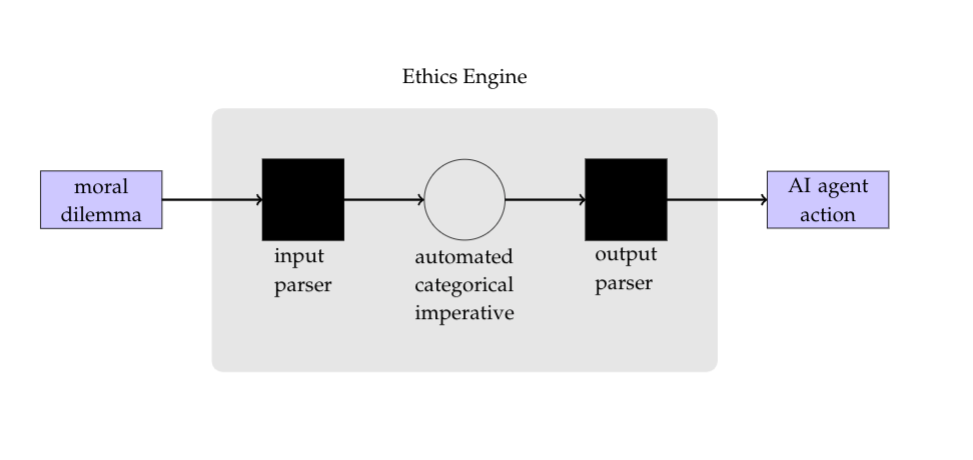
\includegraphics[scale=0.4]{AI_engine.png}
\caption{An example of an ethics engine for an artificial agent. I contribute the automated 
categorical imperative component.} \label{fig:AIengine}
\end{figure}
%
\begin{isamarkuptext}%
In this workflow, an AI agent is faced with a moral dilemma in some internal representation. This 
internal representation would need to be translated by an input parser into an appropriate logical representation, i.e. 
a circumstance, act, goal tuple. This input parser is the most technically and ethically challenging 
component of the system. It is this input parser that determines which circumstances are ``morally relevant"
for a maxim, a judgement that requires commonsense reasoning and knowledge about moral relevance. Translating 
 everyday situations into appropriate maxims is the bulk of the work that a Kantian human being does when making decisions. 
Common misconceptions about Kantian ethics\footnote{For example, some wonder why the FUL doesn't prohibit
gay sex, as the maxim ``marry someone of the same sex" appears to result in human extinction when 
universalized. The solution to this dilemma is that the maxim a gay person acts on is usually something 
of the form, ``marry the person you love because you love them," which is perfectly reasonable to 
universalize.} often result from incorrectly formulated maxims, and the entire field of 
applied Kantian ethics is devoted to generating the right kinds of maxims to test. For more discussion 
of challenges involved with defining morally relevant circumstances, see Section UNWRITTEN.

This representational
question will be one of the biggest hurdles to actually using my categorical imperative library 
in an AI ethics engine. Currently, it may be reasonable for a human being to perform the role of the input
parser. Once an AI agent stumbles onto an ethical dilemma, a human being could take over, formulate 
the right question, and feed it into the categorical imperative library to see what action the categorical 
imperative would prescribe. This may actually be a feature, not a bug. 
Proponents of the ``human-in-the-loop" model argue that fully automated decision-making is doomed 
to ethical failure, and that the inclusion of a human being injects common-sense sanity into otherwise 
dangerous decisions\footnote{For more discussion of different models of AI ethics, see Section UNWRITTEN}.  

It is likely that, regardless of the strengths of the human-in-the-loop model, fully automated AI 
agents will exist. Even if developing this kind of AI is irresponsible,
such developments are likely and will require ethics engines, or risk no consideration of ethics at all. Even if 
fully automated AI is scary, such AI with automated ethics is better than such AI without. 
In such a world, the input parser in my ethics engine would have to be automated. This would require 
that the parser translate the AI agent's internal representation to the appropriate logical representation.
The input parser would need enough common sense reasoning to determine what circumstances are morally 
relevant to a maxim. This is a question that, like all of ethics, philosophers debate robustly
\footnote{\citet{powers} identifies this as a challenge for automating Kantian ethics and briefly sketches 
solutions from \citet{constofreason}, \citet{silber}, and \citet{rawlsconstructivism}. }. 
It is likely that, just as different implementations of automated ethics choose 
a particular ethical theory and implement it, different implementations of such an input parser would 
need to adopt different interpretations of commonsense reasoning and morally relevant circumstances.
Automating this level of commonsense reasoning would represent signifiant technical progress in 
computational ethics.

Once the input has been parsed, either by a human or a machine, into  a sentence in my logic, my 
project can evaluate its moral status using my implementation of 
the FUL. Concretely, my project would return a value indicating if the maxim is obligatory, permissible, 
or prohibited. The maxim would be prohibited if it fails the universalizability test, permissible if it passes, and obligatory 
if its negation fails the universalizability test. All three of these properties amount to testing if a 
certain theorem holds or not in my logic, a calculation that I demonstrate in my tests. 

This output could then be converted into some actionable, useful response with another output parser, 
and then passed back to the AI agent. For example, if the AI agent is equipped to evaluate natural language prescriptions, the 
status of the maxim could be parsed into a natural language sentence. This output will be passed back 
to the AI agent, which will use it to make a decision. The input parser, categorical imperative library, 
and output parser together constitute an ``ethics engine" that AI agents could use as a black box 
implementation of an ethical theory. 

The ethics engine depicted above is a high-level example of one way to use my project to guide an artifical agent. The 
upshot is that an automated version of the categorical imperative could become part of the ethical engine 
for an AI agent, with much work to parse the input and the output. Effectively, the kind 
of automated ethics I implement could be a library that AI developers use to give AI agents the capacity for 
sophisticated ethical reasoning faithful to philosophical literature. This represents an improvement 
over existing ethics engines, which rarely attempt to capture the complexity 
of any ethical theory that philosophers plausibly defend. Moreover, a logic programming approach 
is potentially more explainable than a black-box deep learning approach, as theorem provers like 
Isabelle can explicitly list the axioms used to generate moral prescriptions. For more on how my project 
is situated among other work in automated ethics, see Section Related Work.%
\end{isamarkuptext}\isamarkuptrue%
%
\isadelimdocument
%
\endisadelimdocument
%
\isatagdocument
%
\isamarkupsubsection{Computational Philosophy%
}
\isamarkuptrue%
%
\endisatagdocument
{\isafolddocument}%
%
\isadelimdocument
%
\endisadelimdocument
%
\begin{isamarkuptext}%
Above I explained how my system offers a mechanism for humans to build ethical AI agents. I also 
argue that computational ethics is a mechanism for computers to help humans think differently about 
philosophy. Just as theorem provers make mathematics more efficient and push mathematicians to think 
precisely about the phenomena they are modelling, computational ethics can help philosophers think more precisely about 
philosophy. Below I share a personal example of the kind of philosophical insight that computational ethics 
can prompt and analyze the value that this tool offers to philosophers.%
\end{isamarkuptext}\isamarkuptrue%
%
\isadelimdocument
%
\endisadelimdocument
%
\isatagdocument
%
\isamarkupsubsubsection{Example of a  Philosophical Insight%
}
\isamarkuptrue%
%
\endisatagdocument
{\isafolddocument}%
%
\isadelimdocument
%
\endisadelimdocument
%
\begin{isamarkuptext}%
As I implemented a formalization of the categorical imperative using an interactive theorem prover, 
I discovered logical insights. These logical insights led to a philosophical 
insight that was novel to me and is potentially novel to the field.  While this 
insight could have been reached without the help of the computer, my system's logical results provoked
an interesting philosophical conversation. Effectively, the system spat out a logical principle, and 
I examined the philosophical plausibility of this principle for the ethical 
theory I am formalizing. In this section, I will first present the logical insight, then the 
philosophical insights, and then its implications for a debate about self-doubt. I will then
generalize my personal experience and argue that computational ethics is a new, useful methodology 
for philosophers.

I arrived at the logical insight while testing my formalization of the FUL. I realized
that my formalization was inconsistent unless I specified that the FUL only held for ``well-formed maxims,"
such that neither the act nor goal were already achieved in the given circumstances. Precisely, 
a circumstance, act, goal tuple (c, a, g) is well-formed if $(\neg (c \longrightarrow a) ) \wedge 
(\neg(c \longrightarrow g))$. This provoked the philosophical insight that maxims of this form, in which 
the act or the goal has already been accomplished in the given circumstances are ``vacuous" because 
any prescriptions they generate have already been acted on or violated. The notion of a vacuous maxim
has implications for debates about ethical self-doubt and self-confidence or self-respect.

Below, I document the process used to arrive at the logical insight that the FUL is inconsistent if it
holds for maxims in which $(c \longrightarrow a) \wedge (c \longrightarrow g)$. For those uninterested
in the details of this exploration, it suffices to understand that I used Isabelle to show that if the 
FUL holds for badly formed maxims, then it is inconsistent. After I realized that my formalization was 
inconsistent, I made many failed attempts to diagnose and fix the problem before reaizing that the problem 
lay in badly formed maxims. 

\emph{Logical Insight}

First, I used Sledgehammer to show that my formalization of the FUL\footnote{The full logical representation is \isa{FUL{\isadigit{0}}\ {\isasymequiv}\ {\isasymforall}c\ a\ g\ s{\isachardot}\ not{\isacharunderscore}universalizable\ {\isacharparenleft}c{\isacharcomma}\ a{\isacharcomma}\ g{\isacharparenright}\ s\ {\isasymlongrightarrow}\ {\isasymTurnstile}prohibited\ {\isacharparenleft}c{\isacharcomma}\ a{\isacharcomma}\ g{\isacharparenright}\ s}.}
resulted in a contradiction. Sledgehammer was able to tell me which axioms it used to complete 
this proof, showing me that my formalization contradicted the axiom O\_diamond, which states that an 
obligated term cannot contradict its context\footnote{The full form of the axiom is 
$ O \{ A \vert B \} \longrightarrow \diamond (B \wedge A)$}. 
O\_diamond formalizes the principle ``ought implies can" and requires that if A is obligated in context 
C, that A is possible in context C. I hypothesized that there was some tension between 
the antecedent of the FUL, which states that all agents act on the maxim, and the consequent, 
which states that the maxim is prohibited. If the maxim has already been acted on, then not acting on it
is impossible. Thus, the generated prohibition is impossible to obey, so the ought implies can principle
and axiom O\_diamond are violated.

I then experimented with modifications of the FUL, which I eventually abandoned. I tried universalizing the maxim 
at a world other than the current world and defining non-contradictory maxims, in which the maxim's 
circumstances do not contradict the maxim's act. I noticed that, no matter what modifications I made, 
Nitpick was timing out when looking for a model and Sledgehammer wasn't able to find a proof of
inconsistency. Isabelle's proof tools weren't able to tell me if my modifications were 
consistent or not. I suspected that something about my implementation was too slow, perhaps due to 
my liberal use of quantifiers\footnote{Benzmueller warned me that as 
I added quantifiers to the theory, Isabelle's automated proof tools may start to time out.}. 

Isabelle's model checker Nitpick performs an optimized version of a brute force model search, in which it generates many models
and checks if they satisfy the given maxims. I suspected that Nitpick 
was checking large models that exhausted its 
time limit, especially due to the logical complexity of my theory. 
To reduce the logical complexity, I decided to specify the exact number of maxims 
in the system by passing as an argument to Nitpick the cardinality of my desired model. Nitpick no longer
timed out, but it could not find a satisfying model with cardinality 1, and thus could not demonstrate
that my modified FUL was consisteny.
 This puzzled me, as I felt that I could construct a pencil-and-paper 
model with a single world and term in which my modified formalizations were consistent.

Instead of specifying the cardinality of the model, I decided to tell Nitpick exactly how many 
maxims there were in my system by defining them as constants. I defined a particular 
(circumstance, act, goal) tuple as a constant. Instead of
stating that the FUL held for all maxims, I stated that the FUL held for the specific maxim formed by this tuple.
While before I added the axiom $\forall (c, a, g) \text{\emph{FUL holds for maxim}} (c, a, g)$, I now added constants $(c, a, g)$ 
and added the axiom $\text{\emph{FUL holds for maxim}} (c, a, g)$. By specifying the circumstance, act, and goal 
as constants, I removed the external universal quantifier, thus removing a layer of logical complexity.

To my surprise, Nitpick not only returned quickly, it was able to show that the FUL was consistent!

This result was counterintuitive—after all, what is the difference between a model of cardinality 
1 and a model with one constant object? Why is quantifying over a tiny number of maxims different
 than analyzing a single maxim? Professor Amin pointed out that, as constants, the 
circumstances, act, and goal were all distinct. When they were quantified over, 
they could be identical. To formalize this idea, I defined a maxim as \isa{well{\isacharunderscore}formed\ {\isasymequiv}\ {\isasymlambda}{\isacharparenleft}c{\isacharcomma}\ a{\isacharcomma}\ g{\isacharparenright}\ s\ w{\isachardot}\ {\isasymnot}\ c\isactrlbold {\isasymrightarrow}g\ w\ {\isasymand}\ {\isasymnot}\ c\isactrlbold {\isasymrightarrow}a\ s\ w}. In propositional 
logic, a circumstance, act, goal tuple (c, a, g) is well-formed if $(\neg (c \longrightarrow a) ) \wedge 
(\neg(c \longrightarrow g))$. I tested my hypothesis by modifying my axiom to instead read $\forall$\emph{maxim
(maxim is well-formed} $\longrightarrow$ \emph{FUL holds for maxim}). This version of the FUL was indeed consistent!

To summarize, I realized that my initial attempt at formalizing the FUL was inconsistent because 
it required that the FUL hold for badly formed maxims, in which the circumstances entail the act or 
goal. The logical insight was that if FUL holds for maxims in which $(c \longrightarrow a) \vee 
(c \longrightarrow g)$, then the logic will be inconsistent.

\emph{Philosophical Insight}

Once I realized this logical property, I tried to understand its philosophical plausibility. I 
wanted to philosophically test the hypothesis that maxims in which  $(c \longrightarrow a) \vee 
(c \longrightarrow g)$ are not valid inputs to the FUL. I concluded that because vacuous maxims neither 
change an agent's behavior nor generate meaningful obligations, they are not the right kinds of questions 
for practical reasoners to be asking. They cannot be action-guiding and are thus not the kind of problem that 
ethics should be concerned with. Moreover, under the Kantian account of the will, the very act of asking 
if a vacuous maxim is prohibited generates a contradiction by undermining the will's authority over itself. 

I define a vacuous maxim as one in which the circumstances entail either the act or the goal and argue 
that such maxims can't meaningfully guide action. Consider the example vacuous maxim, ``when eating 
breakfast, I will eat breakfast in order to eat breakfast." This 
maxim isn't clearly obligatory or prohibited, but there is something empty about it. Acting on this
 maxim could never result in any actual action. If an agent adopts this maxim, 
they decide that, in the circumstances ``eating breakfast" they will perform the act ``eating breakfast"
for the purpose ``eating breakfast." In these circumstances, the act has 
already been performed! Treating this maxim a law for yourself or a principle to live by doesn't change 
how you live your life. If you adopt this maxim, when you are eating breakfast, you eat breakfast, 
but this statement is already tautologically true. 

Not only does a vacuous maxim fail to prescribe action, any obligations or prohibitions it 
generates have already been fulfilled or violated. If a vacuous 
maxim generates a prohibition, then this prohibition would be impossible to obey. 
It is impossible to not eat breakfast while eating breakfast, because the circumstances assume that the 
act has happened. On the other hand, if a vacuous maxim generates an obligation, then the obligation 
will have already been fulfilled. If you are required to eat breakfast while eating breakfast, then you've 
already fulfilled your obligation because the circumstances assume that the act has happened. Thus, 
a vacuous maxim does not actually guide action because it doesn't generate new obligations or 
prohibitions that could ever be acted on. 

Because vacuous maxims can't prescribe or alter action, they are not practically action-guiding and 
thus are not the right kinds of maxims for practical reasoners to evaluate. Moreover, insofar as ethics 
is supposed to guide action, vacuous maxims cannot be part of this project. Vacuous maxims
will have no bearing on what someone should do. Practical reason
is the kind of reason that helps us decide what we should do. 
A practical reasoner asks moral questions not as a mental puzzle or out of curiosity, but 
in order to decide how to act. Practical reason is action-guiding, but a vacuous
 maxim can never be action-guiding because it prescribes no new
actions or obligations. It is not the kind of maxim that a practical reasoner should consider, because it
will have no bearing on what the agent should do. 
There is no explicit prohibition against a vacuous maxim like the breakfast example above, but it 
is the wrong kind of question for a practical reasoner to ask. An ordinary person trying 
to navigate the world would never need to ask that kind of question. If ethics is meant 
to guide action, then badly formed maxims are not questions for ethics, because they could never guide 
action.

Above I argued that vacuous maxims are not the kind of principle that a practical reasoner should 
evaluate, and are thus not the right kind of question for ethics. Kantians can make an even stronger claim
about vacuous maxims—because maxims are laws that you give to yourself, asking if you should will 
a maxim as you will it undermines your will's law-giving ability. The circumstances of a vacuous maxim 
already assume that the agent has willed the maxim. Under the Kantian acount of willing, this act 
of willing a maxim is equivalent to giving the maxim to yourself as a law. When you will a maxim, you
adopt a law to make the maxim your end and commit yourself to be its cause. You cannot simultaneously 
commit yourself to a maxim and ask if you should be committing to it. To 
will the maxim is to adopt it as law—so the question, ``should I be 
willing this?" is paradoxical. Either you haven't actually made the maxim your law (and thus haven't yet 
committed yourself to it), or you aren't actually asking the question (because the decision has already been made).
Because a maxim is a law that you give to yourself, you cannot question it absent a sufficient reason 
(such as a change in the circumstances). To question a law arbitrarily is to not regard it as a law at all.
This kind of questioning amounts to questioning the will's authority over itself, but this is 
impossible. The will definitionally has authority over itself, for that is what it is to be a 
will. 

A skeptic may argue that we do often ask ``should I be doing this?" as we do something. What do we mean when 
we ask this question? In what sense are we trying to evalute the moral status of a vacuous maxim?
Can this kind of question ever be valid? To understand this worry, I consider the maxim, 
``When dancing, I should just dance for the sake of dancing."\footnote{Maybe cite Korgsaard since the
dancing thing is her example.} While this maxim appears to be vacuous (the 
circumstance `dancing' implies the act and goal of dancing), it's a question that practical reasoners 
do ask. I argue that there are this maxim is actually misunderstood and, when interpreted correctly,
it no longer poses as a counterexample to my complaints about vacuous maxims.

Under one reading of this maxim, "I should just dance" is actually referring to a different act than the circumstance ``when dancing". 
The circumstance ``when dancing" refers 
to rythmically moving your body to music, but ``I should just dance" refers to dancing without anxiety, 
completely focused on the joy of dancing itself. More precisely, this maxim should read ``When 
dancing, I should abandon my anxiety and focus on dancing for the sake of dancing." This maxim when so 
modified is not vacuous at all—abandoning anxiety and focusing on dancing is an entirely different act 
from moving your body rythmically to music. This maxim is actually well-formed, and thus doesn't
pose a problem for my argument. It is entirely plausible to tell yourself ``When I am dancing, I should focus 
on dancing for the sake of dancing itself." The circumstances do not entail the act or the goal because 
they refer to different meanings of the word dancing. Any valid reading of this maxim will have the structure above, 
in which the act is actually different from the circumstances. A reasoner cannot accept their will 
as law-giving or commit themselves to an act and simultaneously question the act. Either they must be 
questioning a different act or they must have recieved new information to prompt the questioning, 
modifying the circumstances of the original maxim. 

Another related worry has to with maxims that we do in fact think are prohibited. Consider the maxim modified to 
read ``When dancing and seeing a child drowning, I should dance for the sake of dancing." Clearly this 
maxim is fit for moral evaluation, and we expect a moral theory to prohibit this maxim. The circumstances 
``When dancing and seeing a child drowning" appear to entail the act of dancing, and the maxim thus 
appears vacuous. Once again, this maxim is formulated incorrectly. In this case, the question 
that the agent is actually asking themselves is ``should I continue dancing?" That is the 
maxim that they will adopt or reject. They mean to ask if they should stop dancing and go help the child. 
Dancing at the current moment and dancing at the next moment are different acts, and the circumstances 
imply the former but not the latter. A vacuous maxim would have circumstances and act both 
``dancing at moment t," but this maxim has circumstances ``dancing at moment t" and act ``dancing 
at moment t+1." This is a kind of temporal error that has bearings for other debates in ethics as well. 
Specifically, the confusion between circumstances and acts that occur at different times (as in this example) and circumstances 
and acts that occur at the exact same time has bearing on self-doubt, as I will argue next.

\emph{Implications for Self Doubt and Self Respect}

The dancing maxim can also be understood through the lens of self-doubt. Under this 
reading, the question ``When I am dancing, 
should I be dancing for the sake of dancing?" is the agent asking, ``Am I doing the right thing 
right now?" Unlike the drowning example, the agent is not asking about the next moment, but is expressing doubt about the 
moral validity of their behavior at this current moment. I do not want to argue that self-doubt always
 undermines the will—after all, self-doubt plays an important role in moral 
reasoning and is often the mark of a thoughtful agent. I argue instead that questions of self-doubt
do not actually involve vacuous maxims, for these are not the maxims that the agent is doubting. Indeed,
this example demonstrates that the tension between self-doubt and self-respect arises from a 
mistaken characterization of questions of self-doubt as questions about vacuous maxims.
I first explain the tension between self-doubt and self-respect in epistemology, then 
explain the parallel tension in ethics, and finally present a resolution of this tension.

In epistemology, there is a tension between the rational requirement to believe in yourself and the 
value of self-doubt, in moderation. Christensen presents the ``principle of self-respect," which requires 
that any rational agent refrain from believing that they have mistaken beliefs \cite[4]{christensen}. For example, I cannot 
rationally both believe that the sky is blue and believe that I believe that the sky is green. In other words, I cannot 
disapprove of my own credences. Christensen argues that this principle, which he abbreviates to SR, holds because 
a perfectly rational agent can make accurate and confident judgements about what they believe. If this 
is the case, violating SR results in a simple contradiction \cite[8-9]{christensen}. 

While most philosophers accept some version of SR\footnote{Van Fraassen, Vickers, Koons \cite[5]{christensen}}, 
Roush argues that the principle must be modified in order to account for healthy epistemic 
self-doubt. She argues that, while pathological second-guessing is roundly criticized, we are generally 
imperfect beings, and some sensitivity to our own limitations is a virtue \cite[2]{roushselfhelp}. Indeed, even Christensen 
acknowledges that total self-confidence is an epistemic flaw \cite[1]{christensen}. Thus, there is tension between the rational
requirement to respect our authority as believers and the practical reality that we are often wrong. 

This debate between self-respect and self-doubt in epistemology also applies to ethics. When we 
decide to act and commit ourselves to acting, we cannot simultaneously doubt the 
validity of our action. If human behavior is purposive, then the very act of committing oneself implies 
that one has sufficient reasons for committing oneself. These reasons may be flawed, but in making the 
commitment, the reasoner has accepted them. It is contradictory to claim that someone commits and questions 
simultaneously, because commitment itself implies a resolution to the question. Either the commitment 
is not real, or the question is not. I will call the principle that 
one cannot will a maxim and simultaneously question if they should will that maxim
``ethical self-respect" or ESR.

On the other hand, self-doubt is an important part of ethical reasoning. Just as believers are often 
mistaken, so are practical reasoners. An agent with perfect confidence, who is always sure that they 
are doing the right thing, is clearly not thinking deeply enough about their obligations. Some degree
of ethical self-doubt is normal and likely desirable. Thus, there is a tension between the rational
requirement of ESR and the intuitive validity of ethical self-doubt (ESD).

To resolve this tension, I return to my earlier example of a dancer. Imagine Sara is dancing at a 
weddding, when, in a moment of angst, she asks herself, ``Should I really be dancing right now?" 
What question is she asking here? The immediate answer is that she asking if the maxim, ``When dancing 
at your friend's wedding, dance for the sake of dancing" is a permissible maxim to act on. Notice that t
he maxim in question is vacuous: the circumstance ``when dancing at a friend's wedding" implies the act 
``dance." Because this is a vacuous maxim, it cannot be the maxim that she is questioning, for adopting 
this maxim could not have changed her behavior at all. Sara is asking a question about her actions and 
their validity. Any conclusions about the validity of a vacuous maxim would not help her, first because 
the maxim has no effect on her action, and second because any such validity would be a foregone conclusion
as she has already adopted the maxim. As 
I argued above, no practical reasoner can coherently ask themselves whether a vacuous maxim is 
valid or not without undermining their will, which is a contradiction. Thus, under 
the interpretation of self-doubt as a vacuous maxim, the tension between ESR and ethical self-doubt 
appears irresolvable. Those committed to this interpretation must abandon one principle or the other.

To resolve this issue, I turn to another interpretation of ethical self-doubt. Under this interpretation, 
when Sara asks, ``Should I really be dancing right now?" she wants to know if the maxim that 
resulted in the current moment when she is on the dance floor was actually 
the right thing to will. She is asking if she made the right 
decision in the past, when she decided to dance. The maxim that initiated the dancing would be something 
like ``When at a wedding, dance for the sake of dancing." This is the maxim that she is currently acting 
on, not the vacuous maxim ``When dancing, dance for the sake of dancing." Under this interpretation, 
there is no tension at all between self-doubt and self-respect. It is perfectly valid for a reasoner 
to doubt their prior moral judgements, just as it is perfectly rational for a believer to doubt their 
past beliefs \cite[3-4]{christensen}. Such doubt does not undermine the reasoner's decision-making 
capacity and is thus perfectly consistent with ethical self-respect. 

Not only does this second interpretation resolve the tension between ESR and ESD, it also more accurately 
tracks the operation of practical reason. As argued above, a practical reasoner would never ask themselves 
whether or not to will a vacuous maxim, because such a maxim would generate no meaningful obligations. 
Adopting such a maxim would not alter their behavior in any way. Moreover, the fact that a practical 
reasoner never adopts a vacuous maxim demonstrates the cause of the tension between ESR and ESD.
The tension itself arises from a misreading of questions of self-doubt as questions about 
the evaluation of vacuous maxims. A question of self-doubt cannot refer to a vacuous maxim and must 
instead refer to a well-formed maxim about the agent's past decision-making. As seen before, cases where 
agents appear to ask themselves about vacuous maxims are mistaken about the maxim in question, because 
such a question could never yield a useful answer for a practical reasoner.%
\end{isamarkuptext}\isamarkuptrue%
%
\isadelimdocument
%
\endisadelimdocument
%
\isatagdocument
%
\isamarkupsubsubsection{The Value of Computational Ethics%
}
\isamarkuptrue%
%
\endisatagdocument
{\isafolddocument}%
%
\isadelimdocument
%
\endisadelimdocument
%
\begin{isamarkuptext}%
I will now generalize from the personal insight reached above to the methodological value of 
computational ethics for philosophers.
I do not argue that computational ethics, as it stands today, uncovers philosophical insights that humans have not reached
or are incapable of reaching. After all, my understanding of a well-formed maxim could 
very well exist in the literature and certainly could be reached by a philosopher without any 
computational tools. Instead, I argue that computational tools prompt philosophers to ask questions that 
lead to insights. Philosophers already value precision, and the computer forces precision and makes formal
reasoning easier. Computational 
ethics can serve as another tool in a philosopher's arsenal, like a thought experiment or counterexample.
While the technology is not yet mature enough and easy enough to use to become widespread in philosophy
departments, technical progress could turn computational ethics into an easy-to-use tool for philosophers
that doesn't require any specialized progamming or logical knowledge.

The first contribution of computational ethics is precision \footnote{TODO: this article discusses 
benefits of precision: bookmarked}. Much of analytic philosophy involves 
making a particular concept precise. Thought experiments, arguments, counterexamples, and examples 
illustrate features of a concept in the hope of making the concept itself more precise. Computational 
ethics can help philosophers reach this goal of precision in another, potentially easier, way. 
Representing a philosophical idea in logic and implementing it in an interactive theorem prover requires 
making the idea precise to a degree that ordinary discussion can result in, but does not necessarily require. The initial representation 
of an idea in a logic requires making its form precise. For example, 
as I formalized the notion of a maxim, I had to understand its components and define it as a 
circumstance, act, goal tuple. Moreover, Isabelle's strict typing system required that I define 
coherent, consistent types for each of these entities and for a maxim as a whole. This requires understanding 
what role each of these components play in the FUL and assigning them each a type. In my example, I 
concluded that circumstances and goals are terms, which can be true or false at a world, and acts are 
open sentences, which are true for a particular subject at a particular world. This precision is possible 
without computational tools, but computational ethics forces a level of precision that ordinary discussion 
does not demand. Type fuzziness and overloaded definitions are all too common in philosophical writing and 
discussion (would be cool to cite some famous debate revolving around this idea), but computers don't 
allow this kind of imprecision.

Another, related benefit of computational ethics is that it makes formal ethics far less tedious. 
Certain subfields, such as philosophy of language, see such benefit in precision that they already 
use symbolic logic to represent philosophical concepts, just as mathematicians use symbolic logic to 
represent mathematical concepts. Some of this work requres tedious pencil and paper proofs to prove 
theorems, even when many of these theorems may not generate relevant philosophical insights. Interactive 
theorem provers make formal logic more accessible. Isabelle can complete a proof, starting from first principles, 
in a matter of seconds that would take a logician pages to complete. Similarly, Nitpick can generate 
examples or counterexamples to a proposition in a brute force manner. The computer can generate hypotheses
that philosophers can then think about, just as it did for me to prompt the insight above.

Just as calculators make arithmetic more accessible, computational ethics does the same for formal philosophy. 
Not all philosophy can or will 
be formalized or automated—after all, calculators didn't make accountants or mathematicians obsolete. Just as computers 
reduce the tedium in other aspects of our life, they can reduce the tedium involved in formal logic to 
allow mathematicians and philosophers to focus their attention on understanding.%
\end{isamarkuptext}\isamarkuptrue%
%
\isadelimdocument
%
\endisadelimdocument
%
\isatagdocument
%
\isamarkupsubsubsection{Looking Forward%
}
\isamarkuptrue%
%
\endisatagdocument
{\isafolddocument}%
%
\isadelimdocument
%
\endisadelimdocument
%
\begin{isamarkuptext}%
Computational ethics is at its infancy. The use of theorem provers in mathematics is just now beginning 
to make headway \cite{buzzardvideo}, even though theorem provers were first invented in the 1960's \cite{historyofITP}. In contrast, the first attempts to use theorem 
provers for ethics occurred in the last decade. The fact that this nascent technology is already 
helping humans reach non-trivial philosophical conclusions is reason to, at the very least, entertain 
the possibility of a future where computational ethics becomes as normal for philosophers.

To the skeptic, the ethical insights uncovered by the computer are not necessarily impressive 
philosophy. Indeed, the fact that a theorem prover requires specialized knowledge outside of the field 
of philosophy indicates that the technology is nowhere near ready for universal use in philosophy 
departments. However, history indicates that as computing power increases and computer scientists make 
progress, computational ethics will become more usable. Theorem provers in mathematics began as toys 
incapable of proving that the real number 2 is not equal to the real number 1, but Buzzard showed that 
moving from such a primitive system to a tool for Fields medal winning mathematics is possible in a 
matter of years \cite{buzzardvideo}. Countless examples from the history of computer science, from the Turing 
Test to AI game playing to protein folding, demonstrate that progress in computer science can make seemingly 
obscure computer programs useful and usable in ways that exceed our wildest imaginations. Indeed, 
programmable computers themselves initially began as unwieldy punch card readers, but their current ubiquity 
need not be stated. If computer scientists and philosophers invest in computational ethics, it can 
become as much a tool for philosophy as a calculator is for for arithmetic.\footnote{Is this too like, 
lalalala fantasy of computational philosophy? Would it be less so if I did more work explaining 
the history of theorem proving for math? Is this even that important for my project?}%
\end{isamarkuptext}\isamarkuptrue%
%
\isadelimtheory
%
\endisadelimtheory
%
\isatagtheory
%
\endisatagtheory
{\isafoldtheory}%
%
\isadelimtheory
%
\endisadelimtheory
%
\end{isabellebody}%
\endinput
%:%file=~/Desktop/cs91r/paper/upshot.thy%:%
%:%24=6%:%
%:%36=8%:%
%:%37=9%:%
%:%38=10%:%
%:%39=11%:%
%:%40=12%:%
%:%41=13%:%
%:%42=14%:%
%:%43=15%:%
%:%44=16%:%
%:%53=18%:%
%:%65=20%:%
%:%66=21%:%
%:%67=22%:%
%:%68=23%:%
%:%69=24%:%
%:%70=25%:%
%:%71=26%:%
%:%72=27%:%
%:%73=28%:%
%:%74=29%:%
%:%75=30%:%
%:%76=31%:%
%:%77=32%:%
%:%80=36%:%
%:%81=37%:%
%:%82=38%:%
%:%83=39%:%
%:%84=40%:%
%:%85=41%:%
%:%88=43%:%
%:%89=44%:%
%:%90=45%:%
%:%91=46%:%
%:%92=47%:%
%:%93=48%:%
%:%94=49%:%
%:%95=50%:%
%:%96=51%:%
%:%97=52%:%
%:%98=53%:%
%:%99=54%:%
%:%100=55%:%
%:%101=56%:%
%:%102=57%:%
%:%103=58%:%
%:%104=59%:%
%:%105=60%:%
%:%106=61%:%
%:%107=62%:%
%:%108=63%:%
%:%109=64%:%
%:%110=65%:%
%:%111=66%:%
%:%112=67%:%
%:%113=68%:%
%:%114=69%:%
%:%115=70%:%
%:%116=71%:%
%:%117=72%:%
%:%118=73%:%
%:%119=74%:%
%:%120=75%:%
%:%121=76%:%
%:%122=77%:%
%:%123=78%:%
%:%124=79%:%
%:%125=80%:%
%:%126=81%:%
%:%127=82%:%
%:%128=83%:%
%:%129=84%:%
%:%130=85%:%
%:%131=86%:%
%:%132=87%:%
%:%133=88%:%
%:%134=89%:%
%:%135=90%:%
%:%136=91%:%
%:%137=92%:%
%:%138=93%:%
%:%139=94%:%
%:%140=95%:%
%:%141=96%:%
%:%142=97%:%
%:%143=98%:%
%:%144=99%:%
%:%145=100%:%
%:%146=101%:%
%:%147=102%:%
%:%148=103%:%
%:%149=104%:%
%:%150=105%:%
%:%151=106%:%
%:%160=108%:%
%:%172=110%:%
%:%173=111%:%
%:%174=112%:%
%:%175=113%:%
%:%176=114%:%
%:%177=115%:%
%:%186=117%:%
%:%198=119%:%
%:%199=120%:%
%:%200=121%:%
%:%201=122%:%
%:%202=123%:%
%:%203=124%:%
%:%204=125%:%
%:%205=126%:%
%:%206=127%:%
%:%207=128%:%
%:%208=129%:%
%:%209=130%:%
%:%210=131%:%
%:%211=132%:%
%:%212=133%:%
%:%213=134%:%
%:%214=135%:%
%:%215=136%:%
%:%216=137%:%
%:%217=138%:%
%:%218=139%:%
%:%219=140%:%
%:%220=141%:%
%:%221=142%:%
%:%222=143%:%
%:%223=144%:%
%:%224=145%:%
%:%225=146%:%
%:%226=147%:%
%:%227=148%:%
%:%228=149%:%
%:%229=150%:%
%:%230=151%:%
%:%231=152%:%
%:%232=153%:%
%:%233=154%:%
%:%234=155%:%
%:%235=156%:%
%:%236=157%:%
%:%237=158%:%
%:%238=159%:%
%:%239=160%:%
%:%240=161%:%
%:%241=162%:%
%:%242=163%:%
%:%243=164%:%
%:%244=165%:%
%:%245=166%:%
%:%246=167%:%
%:%247=168%:%
%:%248=169%:%
%:%249=170%:%
%:%250=171%:%
%:%251=172%:%
%:%252=173%:%
%:%253=174%:%
%:%254=175%:%
%:%255=176%:%
%:%256=177%:%
%:%257=178%:%
%:%258=179%:%
%:%259=180%:%
%:%260=181%:%
%:%261=182%:%
%:%262=183%:%
%:%263=184%:%
%:%264=185%:%
%:%265=186%:%
%:%266=187%:%
%:%267=188%:%
%:%268=189%:%
%:%269=190%:%
%:%270=191%:%
%:%271=192%:%
%:%272=193%:%
%:%273=194%:%
%:%274=195%:%
%:%275=196%:%
%:%276=197%:%
%:%277=198%:%
%:%278=199%:%
%:%279=200%:%
%:%280=201%:%
%:%281=202%:%
%:%282=203%:%
%:%283=204%:%
%:%284=205%:%
%:%285=206%:%
%:%286=207%:%
%:%287=208%:%
%:%288=209%:%
%:%289=210%:%
%:%290=211%:%
%:%291=212%:%
%:%292=213%:%
%:%293=214%:%
%:%294=215%:%
%:%295=216%:%
%:%296=217%:%
%:%297=218%:%
%:%298=219%:%
%:%299=220%:%
%:%300=221%:%
%:%301=222%:%
%:%302=223%:%
%:%303=224%:%
%:%304=225%:%
%:%305=226%:%
%:%306=227%:%
%:%307=228%:%
%:%308=229%:%
%:%309=230%:%
%:%310=231%:%
%:%311=232%:%
%:%312=233%:%
%:%313=234%:%
%:%314=235%:%
%:%315=236%:%
%:%316=237%:%
%:%317=238%:%
%:%318=239%:%
%:%319=240%:%
%:%320=241%:%
%:%321=242%:%
%:%322=243%:%
%:%323=244%:%
%:%324=245%:%
%:%325=246%:%
%:%326=247%:%
%:%327=248%:%
%:%328=249%:%
%:%329=250%:%
%:%330=251%:%
%:%331=252%:%
%:%332=253%:%
%:%333=254%:%
%:%334=255%:%
%:%335=256%:%
%:%336=257%:%
%:%337=258%:%
%:%338=259%:%
%:%339=260%:%
%:%340=261%:%
%:%341=262%:%
%:%342=263%:%
%:%343=264%:%
%:%344=265%:%
%:%345=266%:%
%:%346=267%:%
%:%347=268%:%
%:%348=269%:%
%:%349=270%:%
%:%350=271%:%
%:%351=272%:%
%:%352=273%:%
%:%353=274%:%
%:%354=275%:%
%:%355=276%:%
%:%356=277%:%
%:%357=278%:%
%:%358=279%:%
%:%359=280%:%
%:%360=281%:%
%:%361=282%:%
%:%362=283%:%
%:%363=284%:%
%:%364=285%:%
%:%365=286%:%
%:%366=287%:%
%:%367=288%:%
%:%368=289%:%
%:%369=290%:%
%:%370=291%:%
%:%371=292%:%
%:%372=293%:%
%:%373=294%:%
%:%374=295%:%
%:%375=296%:%
%:%376=297%:%
%:%377=298%:%
%:%378=299%:%
%:%379=300%:%
%:%380=301%:%
%:%381=302%:%
%:%382=303%:%
%:%383=304%:%
%:%384=305%:%
%:%385=306%:%
%:%386=307%:%
%:%387=308%:%
%:%388=309%:%
%:%389=310%:%
%:%390=311%:%
%:%391=312%:%
%:%392=313%:%
%:%393=314%:%
%:%394=315%:%
%:%395=316%:%
%:%396=317%:%
%:%397=318%:%
%:%398=319%:%
%:%399=320%:%
%:%400=321%:%
%:%401=322%:%
%:%402=323%:%
%:%403=324%:%
%:%404=325%:%
%:%405=326%:%
%:%406=327%:%
%:%407=328%:%
%:%408=329%:%
%:%409=330%:%
%:%410=331%:%
%:%411=332%:%
%:%412=333%:%
%:%413=334%:%
%:%414=335%:%
%:%415=336%:%
%:%416=337%:%
%:%417=338%:%
%:%418=339%:%
%:%419=340%:%
%:%420=341%:%
%:%421=342%:%
%:%422=343%:%
%:%423=344%:%
%:%424=345%:%
%:%425=346%:%
%:%426=347%:%
%:%427=348%:%
%:%428=349%:%
%:%429=350%:%
%:%430=351%:%
%:%431=352%:%
%:%432=353%:%
%:%433=354%:%
%:%434=355%:%
%:%435=356%:%
%:%436=357%:%
%:%437=358%:%
%:%438=359%:%
%:%439=360%:%
%:%440=361%:%
%:%441=362%:%
%:%442=363%:%
%:%443=364%:%
%:%444=365%:%
%:%445=366%:%
%:%446=367%:%
%:%447=368%:%
%:%448=369%:%
%:%449=370%:%
%:%450=371%:%
%:%451=372%:%
%:%452=373%:%
%:%453=374%:%
%:%454=375%:%
%:%455=376%:%
%:%456=377%:%
%:%457=378%:%
%:%458=379%:%
%:%459=380%:%
%:%460=381%:%
%:%461=382%:%
%:%462=383%:%
%:%463=384%:%
%:%464=385%:%
%:%465=386%:%
%:%466=387%:%
%:%467=388%:%
%:%476=392%:%
%:%488=394%:%
%:%489=395%:%
%:%490=396%:%
%:%491=397%:%
%:%492=398%:%
%:%493=399%:%
%:%494=400%:%
%:%495=401%:%
%:%496=402%:%
%:%497=403%:%
%:%498=404%:%
%:%499=405%:%
%:%500=406%:%
%:%501=407%:%
%:%502=408%:%
%:%503=409%:%
%:%504=410%:%
%:%505=411%:%
%:%506=412%:%
%:%507=413%:%
%:%508=414%:%
%:%509=415%:%
%:%510=416%:%
%:%511=417%:%
%:%512=418%:%
%:%513=419%:%
%:%514=420%:%
%:%515=421%:%
%:%516=422%:%
%:%517=423%:%
%:%518=424%:%
%:%519=425%:%
%:%520=426%:%
%:%521=427%:%
%:%522=428%:%
%:%523=429%:%
%:%524=430%:%
%:%525=431%:%
%:%526=432%:%
%:%527=433%:%
%:%528=434%:%
%:%529=435%:%
%:%530=436%:%
%:%531=437%:%
%:%532=438%:%
%:%533=439%:%
%:%534=440%:%
%:%543=443%:%
%:%555=446%:%
%:%556=447%:%
%:%557=448%:%
%:%558=449%:%
%:%559=450%:%
%:%560=451%:%
%:%561=452%:%
%:%562=453%:%
%:%563=454%:%
%:%564=455%:%
%:%565=456%:%
%:%566=457%:%
%:%567=458%:%
%:%568=459%:%
%:%569=460%:%
%:%570=461%:%
%:%571=462%:%
%:%572=463%:%
%:%573=464%:%
%:%574=465%:%
%:%575=466%:%
\newpage 
\section{Why Kant}
%
\begin{isabellebody}%
\setisabellecontext{whykant}%
%
\isadelimtheory
%
\endisadelimtheory
%
\isatagtheory
%
\endisatagtheory
{\isafoldtheory}%
%
\isadelimtheory
%
\endisadelimtheory
%
\isadelimdocument
%
\endisadelimdocument
%
\isatagdocument
%
\isamarkupsection{Why Kantian Ethics%
}
\isamarkuptrue%
%
\endisatagdocument
{\isafolddocument}%
%
\isadelimdocument
%
\endisadelimdocument
%
\begin{isamarkuptext}%
In this thesis, I formalize Kantian ethics. Deontological theories are attractive candidates for formalization
because, as Powers argues, rules are generally computationally tractable. Intuitively, algorithms are 
rules or procedures for problem solving and Kantian ethics, particularly the Formula of Universal Law
appears to be one such procedure. While computers are generally successful at applying rules, I will 
argue that Kantian ethics is within reach for automation because of its formalism specifically. Due to 
this formalism, reasoning about Kantian ethics requires far less knowledge of the world than alternative
theories. Like all ethical reasoning, reasoning with Kantian ethics requires some judgements about what 
circumstances and facts are morally relevant, but I argue that it requires fewer such judgements than 
consequentialism or virtue ethics. I will present Kantian ethics and describe its formal nature, then briefly
present consequentialism and virtue ethics and compare their automatability. 

I do not aim to show that Kantian ethics is the only tractable theory to automate, and I do not claim to present a comprehensive
overview of all consequentialist or virtue ethical theories. Instead, I present a sample of some theories
in each tradition and argue that Kantian ethics is more straightforward to formalize than these samples.
Insofar as my project serves as an early proof-of-concept for computational ethics, I choose to automate
the ethical theory that appears most amenable to automation.%
\end{isamarkuptext}\isamarkuptrue%
%
\isadelimdocument
%
\endisadelimdocument
%
\isatagdocument
%
\isamarkupsubsection{Kantian Ethics%
}
\isamarkuptrue%
%
\endisatagdocument
{\isafolddocument}%
%
\isadelimdocument
%
\endisadelimdocument
%
\begin{isamarkuptext}%
First, I present a brief overview of Kantian ethics. Kant's theory is centered on the idea of 
practical reason, which is the kind of reason that we use practically to decide what to do. In \emph{The 
Groundwork of the Metaphysics of Morals}, Kant's most influential text on ethics, he explains that 
rational beings are unique because we can act ``in accordance with the representations of laws" \cite[4:412]{groundwork}.
A ball thrown into the air acts according to the laws of physics and lacks the ability to ask itself, 
``should I fall back to the ground?" It simply falls. A rational being on the other hand, can ask themselves
``Should I act on this reason? Is this a sufficient reason for acting?" As Korsgaard describes it, when 
choosing which desire to act on, ``it is as if there is something over and above all of your desires, 
somethig which is you, and which chooses which desire to act on" \cite[100]{sources}. Rational beings are
set apart by this reflective capacity. In other words, a rational being's behavior is purposive: their 
actions are guided by practical reason. They have reasons for acting, even when these reasons may be 
opaque to them. The operation of this practical reason is called the will. 

The will operates by willing maxims, which are its percieved reasons for acting. Kant defines a maxim as 
the ``subjective principle of willing," which is the reason that the will \emph{subjectively} gives 
to itself for acting \cite[16, footnote 1]{groundwork}. There is debate about what exactly must be 
included in a maxim, but most philosophers agree that a maxim consists of some combination of circumstances, 
act, and goal\footnote{For more discussion of the definition of a maxim, see Section What Is a Maxim?}.
One example of a maxim is ``When I am hungry, I will eat a doughnut in order to satisfy my sweet tooth." 
When a moral agent wills this maxim, they decide to act on it. They commit themselves to the end in the maxim, 
satisfying your sweet tooth in this case. They represent their action, to themselves, as following the 
principle given by this maxim. It is maxims that Kant evaluates as obligatory or prohibited. He argues that
certain maxims have a form or logical structure that requires any rational agent to will them. 

The form of an obligatory maxim is given by the categorical imperative, Kant's supreme rule of morality. 
An imperative is a command, such as ``Close the door" or "Eat the doughnut in order to satisfy your 
sweet tooth." A categorical imperative holds unconditionally for all rational agents under all 
circumstances. Kant argues that the moral law must be a categorical imperative, for otherwise it would 
not have the force that makes it a moral law \cite[5]{groundwork}. In order for an imperative to be 
categorical, it must be derived from the will's authority over itself. Our wills are free and bound to 
nothing but themselves. The only thing that can have unconditional authority over a rational will is 
the rational will itself. No one can tell me what reasons to act on because I can always ask why I 
should obey their authority. The only authority that I cannot question is the authority of my own 
practica reason. To question this authority is to demand a reason for acting for reasons, which 
concedes the authority of reason itself \cite[23]{velleman}. Therefore, the only possible candidates 
for the categorical imperative are those rules that are required of the will because it is a will. 
The categorical imperative must be a property of practical reason itself.

Armed with this understanding of practical reason, we can now examine what Kant claims is the categorical 
imperative. He presents three ``formulations" or versions of the categorical imperative and goes on to 
argue that all three formulations are equivalent. In this project, I focus on the first formulation,
the Formula of Universal Law, but will briefly present the other two as well. 

The first formulation of the categorical imperative is the
formula of universal law (FUL), which reads, ``act only according to that maxim through which you can 
at the same time will that it become a universal law." $\cite[34]{groundwork}$ This formulation
generates the universalizability test, which ``tests" the moral value of a maxim by 
imagining a world in which it becomes a universal law and attempting to will the maxim in that world.
Velleman presents a concise argument for the FUL. He argues that reason is shared among reasoners. For 
example, all reasoners have equal access to the arithmetic logic that shows that ``2+2=4"\cite[29]{velleman}. The chain of 
reasoning that makes this statement true is not specific to any person, but is universal across people. 
Therefore, if I have sufficient reasont to will a maxim, so will every other rational agent. There is 
nothing special about the operation of my practical reason that other reasoners don't have access to. 
Practical reason is by its very nature shared, so in adopting a maxim, I implicitly state that all reasoners
across time also have reason to adopt that maxim. Therefore, because I act on reasons, I must obey the 
FUL. Notice that this fulfilles the above criterion for a categorical imperative: the FUL is derived from 
a property of practical reason itself and thus derives authority from the will's authority over itself, 
as opposed to some external authority.

The second formulation of the categorical imperative is the formula of humanity (FUH): ``So act that you use humanity, 
in your own person, as well as in the person of any other, always at the same time as an end, never merely 
as a means." $\cite[41]{groundwork}$. This formulation is often understood as requiring us to 
acknowledge and respect the dignity of every other person. The third formulation of the categorical 
imperative is the formula of autonomy (FOA), which Korsgaard summarizes in her introduction to the Groundwork 
as, ``we should so act that we may think of ourselves as legislating universal laws through our 
maxims." $\cite[28]{korsgaardintro}$ While closely related to the FUL, the FOA presents morality as the activity of 
perfectly rational agents in an ideal ``kingdom of ends," guided by what Kant calls the ``laws of freedom."

The above is not meant to serve as a full defense of Kant's ethical theory, as that is outside the scope
of this thesis. Instead, I aim to briefly reconstruct an argument for Kant's ethical theory in the hopes 
of offering context for the implementation of the FUL I present later in the thesis. Additionally, understanding 
the structure of Kant's argument also reveals facts about his theory that make it an ideal candidate 
for formalization.

Kant argues that the categorical imperative, and the FUL in particular, is a formal principle of practical
reason. In other words, the FUL is a property of reason related to the form or structure of a maxim.
It has nothing to do with the circumstances of behavior (beyond those included in a maxim), the agent's
mental state, or any other contingent facts. Instead, it is purely a property of a proposed principle for
action. This formalism makes Kantian ethics an attractive candidate for formalization. While other 
ethical theories often rely on many facts about the world or the actor, Kantian ethics simply relies 
on the form of a given maxim. A computer evaluating a maxim doesn't require any knowledge about the 
world beyond what is contained in a maxim. A maxim is essentially a thin representation of all the knowledge
that a computer needs in order to make a moral judgement. Automating Kantian ethics merely requires 
making the notion of a maxim precise and representing it to the computer. This distinguishes Kantian 
ethics from utilitarianism and virtue ethics, which, as I will argue below, require far more knowledge
about the world or the agent to reach a moral decision.%
\end{isamarkuptext}\isamarkuptrue%
%
\isadelimdocument
%
\endisadelimdocument
%
\isatagdocument
%
\isamarkupsubsection{Consequentialism%
}
\isamarkuptrue%
%
\endisatagdocument
{\isafolddocument}%
%
\isadelimdocument
%
\endisadelimdocument
%
\begin{isamarkuptext}%
A consequentialist ethical theory is, broadly speaking, any ethical theory that evaluates an action by evaluating 
its consequences\footnote{There is long debate about what exactly makes an ethical theory consequentialist \cite{consequentialismsep}. 
For this paper, I will focus on theories that place the moral worth of an act in its the consequences.}. For example, 
utilitarianism is a form of consequentialism in which the moral action 
is the action that results in the best consequences or produces the most good \cite{utilsep}. Different 
consequentialists take different stances on what exactly constitutes a ``good" consequence and how 
we can aggregate or calculate the goodness of a state of affairs. For example, hedonists define 
a good action as one that produces pleasure, and the most good action as the one that produces that most
pleasure or avoids the most pain. 
Unlike consequentialists, Kantians derive the moral worth of an action
from the maxim that is acted on. This maxim is the actor's subjective reason for acting, determined 
at the time of action, not as a later consequence.

Because consequentialism evaluates the state of affairs following an action, this kind of  ethical 
reasoning requires more knowledge
about the state of the world than Kantian ethics. Under a naive version of consequentialism, evaluating 
an action requires perfect knowledge of all consequences following an action. Not only does this require 
a lot of knowledge that the implementor of an automated ethical system likely does not have, it also 
requires answering difficult questions about which consequences were actually caused by an action\footnote
{maybe cite the debate about difficulties in determining causation?}. Most consequentialists do not actually
think that agents need to calculate all the consequences of their actions; plausible consequentialist strategies include stopping 
calculation early because constant calculation paralyzes action and is clearly not a desirable state of affairs,
only evaluating consequences that the agent could reasonably forsee before acting, or the legal notion 
of ``proximate cause," in which the agent is only responsible for the immediate consequences of their 
acts but not of consequences resulting from others' voluntary acts prompted by the agent's original act \cite{consequentialismsep}.
The details of these views are not important for my project, but it is clear that they require far 
more data than Kantian ethics. Even if we cut off the chain of causal reasoning at some point, evaluating 
the consequences of an action is still data-intensive. Even evaluating the first or immediate cause of an
action requires immense knowledge about the state of the world and how it changes. Kantian ethics, on the 
other hand, requires only knowledge about the maxim, not knowledge about the state of the world when 
the maxim is adopted. Consequentialism requires knowledge about the situation in which the act is 
performed and following the act, whereas Kantian ethics merely requires knowledge about the act itself.

The fact that consequentialism requires more knowledge about the world makes it more difficult to formalize.
Automated consequentialist ethics would need to represent complex states of the world and causal chains
in an efficient manner and reason about them. This presents a difficult technical challenge and
impedes the usability of such a system. Automated consequentialist ethics would need to come equipped with 
a large enough database of knowledge about the world to extrapolate the consequences of an actions and
up-to-date information about the state of the world at the moment of action. Not only does collecting 
and representing this data pose a technical challenge, it also creates a larger ``trusted code base" for 
the automated system. Trusting a Kantian ethical reasoner merely requires trusting the logical implementation
of the categorical imperative, but trusting a consequentialist ethical reasoner requires trusting both the
logical machinery that actually evaluates the consequences of an act and the background/situational
knowledge that serves as an input to this machinery. There is much more room for debate about 
the background knowledge/state of the world than there is about the act that the agent performs.
The Kantian ethical reasoner includes room for 
disagreement about the formulation of the maxim being evaluated\footnote{For more on the parsing 
of ethical dilemmas into maxims, see Section AI Ethics}, but the surface of this debate is much smaller
than the surface of an entire database about actions and their consequences. 

Another such debate that an automated consequentialist reasoner would need to take a stance on is 
the question of what qualifies as a ``good consequence." Simple hedonists associate
good with the presence of pleasure and the lack of pain. Preference utiliarians believe that good is 
the satisfaction of desires and is thus related to individuals' preferences, as opposed to some objective
sensation of pleasure or pain. Other consequentialists adopt a pluralistic theory of value, under which 
many different kinds of things are good for different reasons. For example, Moore values beauty and truth 
and other pluralists value justice, love, and freedom (cite). Welfare utilitarians value a person's 
welfare and utilitarians of right value states of affairs in which respect for some set of crucial
rights is maximized \cite{consequentialismsep}.

Most of the above theories of good require that a moral reasoner understand complex features about
individuals' preferences, desires, or sensations in order to evaluate a moral action, making automated
consequentialist ethics difficult. Regardless of the theory of the good, a consequentialist ethical 
reasoner needs to evaluate a state of affairs, which may encompass each involved individual's pleasure, 
preferences, welfare, freedom, rights, or whatever other criteria make a state good. This not only requires
a lot of data as I argued above, it also requires judgements about whether or not a state of affairs 
actually satisifes the relevant criteria for goodness. These judgements are difficult and debateable, 
and any consequentialist decision requires many of these judgements for each individual involved. As 
systems become more complex and involve more people and more acts, making these judgements quickly becomes
difficult, posing a scaling challenge for a consequentialist ethical reasoner. Perfect knowledge of 
tens of thousands of people's pleasure or preferences or welfare or rights is impossible. Either a human being 
assigns values to states of affairs, which quickly becomes difficult to scale, or the machine does, 
which requires massive knowledge and increases room for doubting the system's judgements.

Once an automated consequentialist agent assigns a goodness measurement to each person in a state of affairs, it 
must also calculate an overall goodness measurement for this state of affairs. One approach to assigning
this value is to aggregate each person's individual goodness score into one complete score for a state. 
For example, under a simple welfare model, each person may be assigned a welfare score and the total 
score for a state of affairs may be the sum of the welfare scores for each involved person.
The more complex the theory of the good, the more difficult that aggregation becomes. For example, 
pluralistic theories struggle to explain how different kinds of value can be compared. How do we compare
one unit of beauty to one unit of pleasure? Subjective theories of the good, such as those focused on 
the sensation of pleasure or an individual's preferences, present difficulties in comparing such 
subjective measures. Resolving this debate requires that the automated reasoner make a decision about
one specific aggregation algorithm, but those who disagree with this choice will not trust the reasoner's
moral judgements. 

On the other hand, some consequentialists reject aggregation entirely and instead prefer wholistic
evaluations of a state of affairs. While this approach no longer requires that a reasoner define an 
aggregation algorithm, the reasoner still needs to calculate a goodness measurement for a state of 
affairs. Whereas before the reasoner could restrict analysis to a single person, the algorithm must now 
evaluate an entire state at once, wholistically. Evaluating the goodness of an entire state of affairs is more complicated
than evaluating the goodness of a single person. As consequentialists modulate between aggregation 
and wholistic evaluation, they face a tradeoff between the difficulty of aggregation and the complexity 
of goodness measurements for large units like states of affairs. This tradeoff translates to an automated
consequentialist moral agent. Such an agent either needs to define an aggregation function, thus opening 
the door to those who disagree with this definition, or needs to evaluate the goodness of entire states
of affairs, which is a complex and data-intensive philosophical and technical challenge.

None of the challenges described above are intractable or capture the full literature of 
all variations of consequentialism. I do not argue that consequentialism is 
impossible to automate. Instead, each of the challenges above either makes an automated consequentialist
agent more complex or requires that the developer ``plant certain flags" and take a stance on philosophical
debates. Such points of difficulty also appear in Kantian ethics, and I deal with them throughout this
project (see Section What is a Maxim). These difficulties are present in any ethical theory, but consequentialism
has more points of difficulty than Kantian ethics and is thus more difficult to formalize both computationally
and philosophically. Given that this project is a proof-of-concept and an early attempt to formalize
a philosophically rigorous ethical theory, I choose Kantian ethics because it is the easier theory to 
formalize. Future work could indeed address the challenges above and formalize consequentialism. The more
ethical theories that comptuational tools can handle, the more valuable computational philosophy becomes 
for philosophers and AI agents. My project contributes a formalization of one theory that poses fewer
challenges than others.%
\end{isamarkuptext}\isamarkuptrue%
%
\isadelimdocument
%
\endisadelimdocument
%
\isatagdocument
%
\isamarkupsubsection{Virtue Ethics%
}
\isamarkuptrue%
%
\endisatagdocument
{\isafolddocument}%
%
\isadelimdocument
%
\endisadelimdocument
%
\begin{isamarkuptext}%
The virtue ethical tradition predates even consequentialism and has countless variations. Below
I explain the centrality of virtue and practical wisdom, two common tenets of most virtue ethical theories.

All virtue ethical theories place virtue, or those traits that constitute a good moral character, 
at the center. Virtue ethicists recommend actions based on the character traits that such actions
would help cultivate. A virtue is commonly accepted as a character trait that "makes its possessor
good" \cite{vesep}. For example, under Aristotlean virtue ethics, the virtues are the traits that 
enable human flourishing, or fulfilling the purpose of a human being. Many modern virtue ethicists abandon
Aristotle's notion of a ``purpose" of human beings, and instead define virtue in terms of the characteristic
activity of human beings (in ethical terms, not telelological terms) (cite from gened paper). Just as 
consequentialists must offer a view of which consequences are good, virtue ethicists must offer some 
theory of the virtues which justifies and presents a list of the virtues. Such theories are varied in
the literature, from the classical virtues of courage and temperance to the Buddhist virtue of 
equanimity to Sen's conception of the virtues as capabilites that serve as ``effective opportunities to 
undertake the actions and activities" an agent wants to engage in. An automated virtue ethical agent 
will need to commit to a particular theory of the virtues, opening itself up to criticism from those
who disagree with this theory of the virtues. Unlike Kantian ethics, who generally agree on the meaning of
the FUL, virtue ethicists robustly debate which character traits qualify as virtues.  

Another difficulty with automating virtue ethics is that the unit of evaluation for a virtue ethical
theory is often a person's entire character. While Kantians evaluate the maxim of an act and utilitarians
evaluate the consequences of an act, virtue ethicists evaluate the actor's moral character and their 
disposition towards the act. Virtues are character traits and evaluating an action as virtuous or 
not requires understanding the agent's character and disposition while acting. If states of affairs
require complex representations, an agent's ethical character and disposition is even more difficult
to represent. Consequentialism posed a data-collection problem in evaluating and representing states
of affairs, but virtue ethics poses a conceptual problem about the formal nature of moral character.
Formalizing the concept of character appears to require significant philosophical and computational
progress, whereas Kantian ethics automatically presents a formal rule to implement. Precise representations
of consequences is a central debate in consequentialism, but precise representation of moral character
is not a central debate in virtue ethics. 

One potential appeal of virtue ethics is that many virtue ethical theories involve some form of 
moral education. Artistotle, for example, argued that cultivating virtuous action requires making such
action habitual through moral education. Under the simple, popular view of virtue ethics, the virtuous
act is what the virtuous person would do. Both of these theories imply that ethical behavior can be
learned from some dataset of virtuous behavior, either those prescribed by a moral teacher or those that
a virtuous ideal agent would undertake. Indeed, these theories seem to point towards a machine learning
model for computational ethics, in which ethics is learned from a dataset of acts tagged as ethical
or not ethical. Such approaches exist in the literature and there is a solid body of work attempting 
to learn ethics from past judgements. My project present a different, top-down approach starting 
with an ethical theory and representing it in a logic. Both approaches have their merits, but one 
advantage of my logical approach is that it does not suffer many of the explainability problems that machine learning 
approaches may experience. Many machine learning algorithms cannot sufficiently explain their decisions
to a human being, and often find patterns or correlations in datasets that don't actually cohere with 
the trends and causes that a human being would identify. While there is significant activity and progress
in explainable machine learning, interactive theorem provers are designed to be explainable at the outset.
Indeed, Isabelle can even give the axioms and lemmas it used in constructing a proof, allowing a human 
being to reconstruct the proof independently if they wish. This is, again, not an intractable problem 
for machine learning approaches to computational ethics, but is one reason to prefer logical approaches.

Explainability matters more for ethics.%
\end{isamarkuptext}\isamarkuptrue%
%
\isadelimtheory
%
\endisadelimtheory
%
\isatagtheory
\isacommand{end}\isamarkupfalse%
%
\endisatagtheory
{\isafoldtheory}%
%
\isadelimtheory
%
\endisadelimtheory
\isanewline
%
\end{isabellebody}%
\endinput
%:%file=~/Desktop/cs91r/paper/whykant.thy%:%
%:%24=6%:%
%:%36=8%:%
%:%37=9%:%
%:%38=10%:%
%:%39=11%:%
%:%40=12%:%
%:%41=13%:%
%:%42=14%:%
%:%43=15%:%
%:%44=16%:%
%:%45=17%:%
%:%46=18%:%
%:%47=19%:%
%:%48=20%:%
%:%49=21%:%
%:%50=22%:%
%:%51=23%:%
%:%60=26%:%
%:%72=28%:%
%:%73=29%:%
%:%74=30%:%
%:%75=31%:%
%:%76=32%:%
%:%77=33%:%
%:%78=34%:%
%:%79=35%:%
%:%80=36%:%
%:%81=37%:%
%:%82=38%:%
%:%83=39%:%
%:%84=40%:%
%:%85=41%:%
%:%86=42%:%
%:%87=43%:%
%:%88=44%:%
%:%89=45%:%
%:%90=46%:%
%:%91=47%:%
%:%92=48%:%
%:%93=49%:%
%:%94=50%:%
%:%95=51%:%
%:%96=52%:%
%:%97=53%:%
%:%98=54%:%
%:%99=55%:%
%:%100=56%:%
%:%101=57%:%
%:%102=58%:%
%:%103=59%:%
%:%104=60%:%
%:%105=61%:%
%:%106=62%:%
%:%107=63%:%
%:%108=64%:%
%:%109=65%:%
%:%110=66%:%
%:%111=67%:%
%:%112=68%:%
%:%113=69%:%
%:%114=70%:%
%:%115=71%:%
%:%116=72%:%
%:%117=73%:%
%:%118=74%:%
%:%119=75%:%
%:%120=76%:%
%:%121=77%:%
%:%122=78%:%
%:%123=79%:%
%:%124=80%:%
%:%125=81%:%
%:%126=82%:%
%:%127=83%:%
%:%128=84%:%
%:%129=85%:%
%:%130=86%:%
%:%131=87%:%
%:%132=88%:%
%:%133=89%:%
%:%134=90%:%
%:%135=91%:%
%:%136=92%:%
%:%137=93%:%
%:%138=94%:%
%:%139=95%:%
%:%140=96%:%
%:%141=97%:%
%:%142=98%:%
%:%143=99%:%
%:%144=100%:%
%:%145=101%:%
%:%146=102%:%
%:%147=103%:%
%:%148=104%:%
%:%149=105%:%
%:%150=106%:%
%:%151=107%:%
%:%152=108%:%
%:%153=109%:%
%:%154=110%:%
%:%155=111%:%
%:%156=112%:%
%:%157=113%:%
%:%166=116%:%
%:%178=118%:%
%:%179=119%:%
%:%180=120%:%
%:%181=121%:%
%:%182=122%:%
%:%183=123%:%
%:%184=124%:%
%:%185=125%:%
%:%186=126%:%
%:%187=127%:%
%:%188=128%:%
%:%189=129%:%
%:%190=130%:%
%:%191=131%:%
%:%192=132%:%
%:%193=133%:%
%:%194=134%:%
%:%195=135%:%
%:%196=136%:%
%:%197=137%:%
%:%198=138%:%
%:%199=139%:%
%:%200=140%:%
%:%201=141%:%
%:%202=142%:%
%:%203=143%:%
%:%204=144%:%
%:%205=145%:%
%:%206=146%:%
%:%207=147%:%
%:%208=148%:%
%:%209=149%:%
%:%210=150%:%
%:%211=151%:%
%:%212=152%:%
%:%213=153%:%
%:%214=154%:%
%:%215=155%:%
%:%216=156%:%
%:%217=157%:%
%:%218=158%:%
%:%219=159%:%
%:%220=160%:%
%:%221=161%:%
%:%222=162%:%
%:%223=163%:%
%:%224=164%:%
%:%225=165%:%
%:%226=166%:%
%:%227=167%:%
%:%228=168%:%
%:%229=169%:%
%:%230=170%:%
%:%231=171%:%
%:%232=172%:%
%:%233=173%:%
%:%234=174%:%
%:%235=175%:%
%:%236=176%:%
%:%237=177%:%
%:%238=178%:%
%:%239=179%:%
%:%240=180%:%
%:%241=181%:%
%:%242=182%:%
%:%243=183%:%
%:%244=184%:%
%:%245=185%:%
%:%246=186%:%
%:%247=187%:%
%:%248=188%:%
%:%249=189%:%
%:%250=190%:%
%:%251=191%:%
%:%252=192%:%
%:%253=193%:%
%:%254=194%:%
%:%255=195%:%
%:%256=196%:%
%:%257=197%:%
%:%258=198%:%
%:%259=199%:%
%:%260=200%:%
%:%261=201%:%
%:%262=202%:%
%:%263=203%:%
%:%264=204%:%
%:%265=205%:%
%:%266=206%:%
%:%267=207%:%
%:%268=208%:%
%:%269=209%:%
%:%270=210%:%
%:%271=211%:%
%:%272=212%:%
%:%273=213%:%
%:%274=214%:%
%:%275=215%:%
%:%276=216%:%
%:%277=217%:%
%:%278=218%:%
%:%279=219%:%
%:%280=220%:%
%:%281=221%:%
%:%282=222%:%
%:%283=223%:%
%:%284=224%:%
%:%285=225%:%
%:%286=226%:%
%:%287=227%:%
%:%288=228%:%
%:%289=229%:%
%:%298=232%:%
%:%310=234%:%
%:%311=235%:%
%:%312=236%:%
%:%313=237%:%
%:%314=238%:%
%:%315=239%:%
%:%316=240%:%
%:%317=241%:%
%:%318=242%:%
%:%319=243%:%
%:%320=244%:%
%:%321=245%:%
%:%322=246%:%
%:%323=247%:%
%:%324=248%:%
%:%325=249%:%
%:%326=250%:%
%:%327=251%:%
%:%328=252%:%
%:%329=253%:%
%:%330=254%:%
%:%331=255%:%
%:%332=256%:%
%:%333=257%:%
%:%334=258%:%
%:%335=259%:%
%:%336=260%:%
%:%337=261%:%
%:%338=262%:%
%:%339=263%:%
%:%340=264%:%
%:%341=265%:%
%:%342=266%:%
%:%343=267%:%
%:%344=268%:%
%:%345=269%:%
%:%346=270%:%
%:%347=271%:%
%:%348=272%:%
%:%349=273%:%
%:%350=274%:%
%:%351=275%:%
%:%352=276%:%
%:%353=277%:%
%:%354=278%:%
%:%355=279%:%
%:%356=280%:%
%:%357=281%:%
%:%358=282%:%
%:%359=283%:%
%:%360=284%:%
%:%361=285%:%
%:%369=289%:%
%:%377=289%:%
\newpage 
%
\begin{isabellebody}%
\setisabellecontext{whycomputationalethics}%
%
\isadelimtheory
%
\endisadelimtheory
%
\isatagtheory
%
\endisatagtheory
{\isafoldtheory}%
%
\isadelimtheory
%
\endisadelimtheory
%
\isadelimdocument
%
\endisadelimdocument
%
\isatagdocument
%
\isamarkupsection{Is Computational Ethics A Good Idea?%
}
\isamarkuptrue%
%
\endisatagdocument
{\isafolddocument}%
%
\isadelimdocument
%
\endisadelimdocument
%
\begin{isamarkuptext}%
Even if computational tools can help philosophers with ethical inquiry, some may worry that they
somehow cheapen philosophy. If there is something valuable about the process of ethical
reasoning, then computational ethics threatens to destroy this value. In this section, I argue that, 
regardless of where we locate the value of ethics, computational ethics can enhance its value. Because
there is some value in human ethical reasoning, we should not completely automate the study of ethics, but 
human-computer symbiotic ethics can preserve and enhance this value. Human-computer symbiosis is a model of computation
in which humans ``set the goals, formulate the hypotheses, determine the criteria, and perform the evaluations,”
and computers perform ``routinizable work that must be done to prepare the way for insights and decisions” \citep{licklider}.
There are two different kinds of ethics that
could benefit from computational tools: the kind that ordinary people use to decide how to live their 
lives and the kind studied by professional philosophers. In the first subsection, I consider the role of ethics 
in an ordinary person’s life and in the second subsection, I analyze the value that ethical study offers to 
the professional philosopher. 

I will contrast human-symbiotic ethics with fully automated ethics, in which computers replace human
ethicists entirely and produce ethical theories and truths with no human input. This vision is far
from becoming a reality. Fully automated ethics may not even be possible, and I do not claim to implement 
anywhere near fully automated ethics in this project. I will use this as an extreme example to understand
the limitations of the arguments below. If a theory of the value of ethical study implies that 
fully automated ethics is good, then it will certainly imply that the kind of ethics I implement
in this project is good.%
\end{isamarkuptext}\isamarkuptrue%
%
\isadelimdocument
%
\endisadelimdocument
%
\isatagdocument
%
\isamarkupsubsection{Ethics for Ordinary People%
}
\isamarkuptrue%
%
\endisatagdocument
{\isafolddocument}%
%
\isadelimdocument
%
\endisadelimdocument
%
\begin{isamarkuptext}%
Ethics has immediate bearing on everyone’s lives because it studies the unavoidable question: 
how should we live? If computers can make this study more efficient, then it seems that everyone should
engage in computational ethics. As Cornel West says, the ethical question is the only question that 
we answer merely by living. To turn away from ethics is to take a stance on the question of how to 
live (namely, to live unreflectively) and thus to engage in ethics. Ethical truths are valuable because 
they tell us how to live. Every rational being must decide how to navigate the world and ethical 
truths answer these questions. If the results of ethical study is practically valuable, then automated 
ethics is good because computational tools can help us locate ethical prescriptions and theories more efficiently. 
In the most extreme case, we can unthinkingly follow the commands of an ethical calculator that dictates 
how we should live. Computers can answer the unavoidable question for us.

Placing the value of ethics solely in its action-guiding potential fails to take into account the 
importance of practical reason, which, as I argued in Section Why Kant, is the source
of freedom itself. 
We are committed to ethical reflection because of the kind of beings that we are. Recall that Korsgaard 
argues that, as beings occupying minds with a reflective structure, when faced with a choice, “it is as if there 
were something over and above all of your desires, something that is you, and that chooses which desire 
to act on” (Sources 83). This choosing is the operation of practical reason, and this reflection
makes us free. We are free because we must choose which reasons to act on. Every decision that we 
make is an exercise of freedom. 

If reflecting makes us free, then unthinkingly obeying the computer sacrifices our autonomy. Consider 
the thought experiment of an Ethics Oracle that can unfailingly tell you the right thing to do in any 
situation.\footnote{This example is inspired by the Pocket Oracle presented in \citet{bok}.} Someone 
who surrenders themselves to this Oracle unthinkingly follows its prescriptions. 
There is some reflection involved in the decision to obey each of the Oracle’s prescriptions, but 
this is a thin kind of reflection \citep{bok}. This person is not reflecting on the real matters at hand and is 
not making decisions for themselves. They have surrendered their reflective capacity to the Oracle. 
They live a worse life than someone who reflects on their actions; they have less ownership over their 
actions than the reflective person. In a less extreme case, a person may retain control of many of 
their decisions but cede some important or tricky choices to the Ethics Oracle. Because every single 
exercise of practical reason is an exercise of autonomy, this person is still less autonomous than the 
purely reflective person. Even surrendering simple, inconsequential decisions such as which flavor of 
coffee to drink surrenders some piece of our autonomy. Perhaps in trivial cases we can accept that 
tiny sacrifice in autonomy, but giving over life-changing decisions to the machine sacrifices our 
core freedom. Unreflectively relying on computational ethics surrenders our autonomy to the machine. 

One objection to this emphasis on reflection is the impracticality of making ethical calculations from first principles 
every time we are faced with a decision. This is why we follow the advice of moral mentors, like our 
family or influential philosophers. These moral mentors differ from the Ethics Oracle because their advice 
comes with an argument justifying it; if human-computer symbiotic computational ethics also prompts 
reflection on the prescriptions given, it can also guide action without sacrificing autonomy.
Most people do not reason about ethics during everyday decisions; they rely on some combination of 
prior knowledge and external testimony. For example, my mother taught me to respect myself, and I 
follow her advice. What is the difference between following the guidance of a moral educator and 
obeying the Ethics Oracle? The best kind of ethical advice prompts reflection, such as an argument 
made in a philosophy paper. Unthinkingly following someone’s advice results in the same loss of 
autonomy as unthinkingly obeying the Ethics Oracle; people who merely obey orders are less autonomous 
than those who think for themselves.\footnote{This might be worrying....does this mean that soldiers who are
following orders to commit atrocities are less responsible than those giving the orders? Wait 
maybe that's true.} This account of moral advice offers a model for human-computer 
symbiotic ethics. The computer should serve as a moral guide by providing arguments, just as my mom 
explained why I should always respect myself. Human-computer symbiotic 
ethics nurtures autonomy when it not only offers prescriptions for action, but also explanations for 
these prescriptions. Because my theorem-prover-based computational ethical system is explainable, it can 
guide action without sacrificing autonomy. It can make an argument for some action, instead of 
merely giving a verdict. Isabelle can list the facts used to show
a partcular action prohibited, and a human being can reflect on whether or not these principles
indeed prohibit the action in question. The computer serves as a collaborator and a tool, but not as an authority, 
so the human being’s reflective capacity and freedom is preserved.%
\end{isamarkuptext}\isamarkuptrue%
%
\isadelimdocument
%
\endisadelimdocument
%
\isatagdocument
%
\isamarkupsubsection{Academic Ethics%
}
\isamarkuptrue%
%
\endisatagdocument
{\isafolddocument}%
%
\isadelimdocument
%
\endisadelimdocument
%
\begin{isamarkuptext}%
There are two potential sources of the value of academic philosophy: the ethical truths uncovered and 
the process of a philosopher discovering these truths. Under the first view, academic philosophy is 
valuable because it facilitates the discovery of new ethical theories. If truths are valuable and 
computers can generate truths more efficiently than humans, then ethics should be fully automated. 
Ethical disputes often linger unresolved indefinitely, but every now and then, 
a theory emerges as a new classic, such as Rawls’ veil of ignorance. Some academic philosophy also 
impacts social phenomena, like Locke’s impact on global democracy. Academic philosophy often works its 
way into household ethics, as seen in the impact of critical race theory. This view parallels the 
view that ordinary ethics is valuable for its insights alone, and thus
similarly implies that totally automated ethics is not only permissible, but also desirable. If 
ethical truths are important for their impact on society, this value is not contingent on whether a 
human or a computer produced these truths. If possible, computers should produce ethical theories 
to maximize these truths’ value for society. 

Another set of theories locates the value of academic ethics in the process itself and thus requires 
human-computer symbiosis. Just as mathematics is fun and creative for the mathematician, so is ethics 
for the philosopher. Many philosophers enjoy reading and writing philosophy papers. The study of 
philosophy builds critical thinking skills and makes philosophers more reflective. Computational ethics 
doesn’t necessarily sacrifice any of these benefits. These 
benefits would be lost by fully automated ethics, but human-computer symbiotic ethics amplifies them. 
If a computer functions like a tool in the process of philosophical discovery, like a conversation 
with a colleague or a search for counterexamples, then it preserves the joy of philosophy. Moreover, 
computational ethics amplifies this joy by forcing ethicists to make their ideas more precise, a major 
goal of academic philosophy. The rigid syntax of a computer program demands much more precision than a 
conversation or a paper. Computational tools also offer ethicists new perspective by forcing a return to 
first, formal principles often avoided in ordinary philosophical inquiry. Formal ethics has been a 
subject of interest among ethicists, but the logical background necessary has prevented the field 
from taking off. If computers can automate away the tedium of formal ethics, then this precision 
will be accessible to all ethicists, not just logicians. Such work has begun in metaphysics, and 
recent research used computational tools to find an inconsistency in Godel’s ontological argument 
for the existence of God \citep{godelincon}. The power of computational tools to force precision, perform 
consistency checks, and make assumptions explicit means that computers can serve as tools to 
help philosophers perform philosophy better.

If ethical truths offer some value to society at-large, perhaps we cannot sacrifice this value merely 
to preserve human philosophers’ fun. A more compelling argument against fully automated 
ethics is that the existence of human academic philosophers offers value even to non-philosophers. 
People derive joy and wonder from knowing that human beings produced great ethics. Plato’s \emph{Apology} 
is not only a profound and insightful text, but it is also wonderous that a human being produced such 
a work. We derive joy from knowing that our fellow humans are capable of the kind of thought that 
great philosophers accomplish, just as an unimaginably beautiful work of art is more wonderous 
because a human being painted it. We watch the Olympics because we derive wonder and joy from human 
excellence. Even when admiring computational achievements, such as Google’s recent success in protein 
folding, we admire the human who programmed the machine, not the machine itself. We can relate to 
humans, so the mere knowledge that great people are doing great things enriches our lives. This 
knowledge is part of the attraction for the thousands of tourists who visit Harvard Yard every year; 
this is a place where of great human achievement.\footnote{Is this too like, yay Harvard}

An even stronger argument for human-computer symbiotic ethics instead of fully automated ethics is 
that ethics is an inherently human subject. We study ethics because, as argued above, we 
have no choice but to reflect on how to live. Because reflection is such a fundamental part of being 
human, a world in which all ethical inquiry is automated is undesirable. Academic philosophers are 
professional reflectors who are partners in the human experience with us, so their ethical inquiry 
carries unique weight. They teach us, inspire us, and serve as examples of the kind of reflection 
that is constitutive of being human. Moreover, an ethical theory produced entirely by a computer is, 
at best, a secondary perspective; it is a computer’s attempt to describe how human beings should live. 
Without a human component, it cannot serve as a rich and sophisticated guide for humans. If ethics is 
most meaningful when it is the product of human reflection, totally automated ethics destroys the field 
entirely but human-computer symbiosis does not. Human beings should debate the most pressing questions 
of human existence, and computers can serve as our aids. Thus, computational tools must supplement 
human ethical reasoning but cannot replace it.%
\end{isamarkuptext}\isamarkuptrue%
%
\isadelimtheory
%
\endisadelimtheory
%
\isatagtheory
%
\endisatagtheory
{\isafoldtheory}%
%
\isadelimtheory
%
\endisadelimtheory
%
\end{isabellebody}%
\endinput
%:%file=~/Desktop/cs91r/paper/whycomputationalethics.thy%:%
%:%24=6%:%
%:%36=8%:%
%:%37=9%:%
%:%38=10%:%
%:%39=11%:%
%:%40=12%:%
%:%41=13%:%
%:%42=14%:%
%:%43=15%:%
%:%44=16%:%
%:%45=17%:%
%:%46=18%:%
%:%47=19%:%
%:%48=20%:%
%:%49=21%:%
%:%50=22%:%
%:%51=23%:%
%:%52=24%:%
%:%53=25%:%
%:%54=26%:%
%:%55=27%:%
%:%56=28%:%
%:%65=31%:%
%:%77=33%:%
%:%78=34%:%
%:%79=35%:%
%:%80=36%:%
%:%81=37%:%
%:%82=38%:%
%:%83=39%:%
%:%84=40%:%
%:%85=41%:%
%:%86=42%:%
%:%87=43%:%
%:%88=44%:%
%:%89=45%:%
%:%90=46%:%
%:%91=47%:%
%:%92=48%:%
%:%93=49%:%
%:%94=50%:%
%:%95=51%:%
%:%96=52%:%
%:%97=53%:%
%:%98=54%:%
%:%99=55%:%
%:%100=56%:%
%:%101=57%:%
%:%102=58%:%
%:%103=59%:%
%:%104=60%:%
%:%105=61%:%
%:%106=62%:%
%:%107=63%:%
%:%108=64%:%
%:%109=65%:%
%:%110=66%:%
%:%111=67%:%
%:%112=68%:%
%:%113=69%:%
%:%114=70%:%
%:%115=71%:%
%:%116=72%:%
%:%117=73%:%
%:%118=74%:%
%:%119=75%:%
%:%120=76%:%
%:%121=77%:%
%:%122=78%:%
%:%123=79%:%
%:%124=80%:%
%:%125=81%:%
%:%126=82%:%
%:%127=83%:%
%:%128=84%:%
%:%129=85%:%
%:%130=86%:%
%:%131=87%:%
%:%132=88%:%
%:%133=89%:%
%:%134=90%:%
%:%135=91%:%
%:%136=92%:%
%:%145=95%:%
%:%157=98%:%
%:%158=99%:%
%:%159=100%:%
%:%160=101%:%
%:%161=102%:%
%:%162=103%:%
%:%163=104%:%
%:%164=105%:%
%:%165=106%:%
%:%166=107%:%
%:%167=108%:%
%:%168=109%:%
%:%169=110%:%
%:%170=111%:%
%:%171=112%:%
%:%172=113%:%
%:%173=114%:%
%:%174=115%:%
%:%175=116%:%
%:%176=117%:%
%:%177=118%:%
%:%178=119%:%
%:%179=120%:%
%:%180=121%:%
%:%181=122%:%
%:%182=123%:%
%:%183=124%:%
%:%184=125%:%
%:%185=126%:%
%:%186=127%:%
%:%187=128%:%
%:%188=129%:%
%:%189=130%:%
%:%190=131%:%
%:%191=132%:%
%:%192=133%:%
%:%193=134%:%
%:%194=135%:%
%:%195=136%:%
%:%196=137%:%
%:%197=138%:%
%:%198=139%:%
%:%199=140%:%
%:%200=141%:%
%:%201=142%:%
%:%202=143%:%
%:%203=144%:%
%:%204=145%:%
%:%205=146%:%
%:%206=147%:%
%:%207=148%:%
%:%208=149%:%
%:%209=150%:%
%:%210=151%:%
%:%211=152%:%
%:%212=153%:%
%:%213=154%:%
%:%214=155%:%
%:%215=156%:%
%:%216=157%:%
%:%217=158%:%
\newpage



% optional bibliography
%\bibliographystyle{apalike}
\bibliography{root}
\end{document}

%%% Local Variables:
%%% mode: latex
%%% TeX-master: t
%%% End:
